%%%%%%%%%%%%%%%%%%%%%%%%%%%%%%%%%%%%%%%%%%%%%%%%%%%%%%%%%%%%%%%%%%%%%%%%%%%%%%%%
\documentclass[12pt]{article}

\special{papersize=8.5in,11in}

\usepackage{cite}
\usepackage{color}
\usepackage{epsfig}
%\usepackage{pslatex}
\usepackage{bm}
\usepackage{xspace}
\usepackage{amsmath}
\usepackage{amssymb}
\usepackage{amsbsy}
\usepackage{eucal}
\usepackage{mathrsfs}


%======================================================
\usepackage{color}
\newcommand{\todo}[1]{\textcolor{red}{#1}}            % material to revise
%\newcommand{\todo}[1]{}  % this makes revise comments disappear
\newcommand{\strike}[1]{\textcolor{magenta}{\sout{#1}}} % material to omit
\newcommand{\comment}[1]{\textcolor{blue}{[ \sc{#1} ]}} % comments
%\newcommand{\comment}[1]{}
%\newcommand{\add}[1]{\textcolor{cyan}{\bf{#1}}}         % recent
%                                % adds/mods
\newcommand{\instructions}[1]{\textcolor{green}{\bf{#1}}}         % instructions to authors
\newcommand{\thoughts}[1]{\textcolor{cyan}{\bf{[#1]}}}         % brainstorming, notes, ...
%\newcommand{\instructions}[1]{}
%\newcommand{\thoughts}[1]{}

\def\btodo{\color{red}}
\def\etodo{\normalcolor\xspace}

\def\bzap{\color{black}}
\def\ezap{\normalcolor}

\newcommand{\invisible}[1]{}

%======================================================

\newcommand{\bi}{\begin{itemize}}
\newcommand{\ei}{\end{itemize}}
\newcommand{\be}{\begin{equation}}
\newcommand{\ee}{\end{equation}}
\newcommand{\bea}{\begin{eqnarray}}
\newcommand{\eea}{\end{eqnarray}}
\newcommand{\bean}{\begin{eqnarray*}}
\newcommand{\eean}{\end{eqnarray*}}
\newcommand{\ben}{\begin{equation*}}		% eqn w/no number
\newcommand{\een}{\end{equation*}}
%\newcommand{\ben}{\[}
%\newcommand{\een}{\]}
\newcommand{\bri}{\begin{redItemize}}
\newcommand{\eri}{\end{redItemize}}

%======================================================

\newcommand{\iid}{\textit{i.i.d.}\xspace}
\newcommand{\etal}{\textit{et al.}\xspace}
\newcommand{\eg}{\textit{e.g.}\xspace}
\newcommand{\ie}{\textit{i.e.}\xspace}
\newcommand{\etc}{\textit{etc.}\xspace}

%======================================================

%\newcommand\RR{{\rm I\kern-.16em R}}


\renewcommand{\thefootnote}{\fnsymbol{footnote}}

\newcommand{\wh}{\widehat}
\newcommand{\p}{\partial}
\newcommand{\dd}{\mathrm{d}}


%\usepackage{amsbsy}
\def\bu{\boldsymbol{u}}
\def\bv{\boldsymbol{v}}
\def\bw{\boldsymbol{w}}
\def\w{\underline{w}}
\def\u{\underline{u}}
\def\v{\underline{v}}
\def\n{\underline{n}}
\def\k{\underline{k}}

\def\TT{\mathrm{T}}
\def\GG{\mathrm{G}}
\def\SS{\mathrm{S}}
\def\VV{\mathrm{V}}
\def\EE{\mathrm{E}}
\def\RR{\mathbb{R}}



\def\co2{{\rm CO}_2}

\def\H{{\rm H}}
\def\Hp{{\rm H}^+}
\def\pH{{\rm pH}}
\def\P{{\rm P}}
\def\D{{\rm D}}
\def\I{{\rm I}}
\def\R{{\rm R}}
\def\L{{\rm L}}
\def\OH{\rm OH}
\def\OHm{{\rm OH}^-}
\def\chemrightarrow#1#2{\,\,\,\smash{\mathop{\longrightarrow}\limits^{#1}_{#2}}\,\,\,}
\def\chemequilarrow#1#2{\,\,\,\smash{\mathop{\longleftrightarrow}\limits^{#1}_{#2}}\,\,\,}
\def\Pa{{\rm H}_3{\rm PO}_4}
\def\Pb{{\rm H}_2{\rm PO}_4^{-}}
\def\Pc{{\rm H}{\rm PO}_4^{2-}}
\def\Pd{{\rm PO}_4^{3-}}
\def\cHp{[\H^+]}
\def\cPa{[\Pa]}
\def\cPb{[\Pb]}
\def\cPc{[\Pc]}
\def\cPd{[\Pd]}
\def\K{{\rm K}}
\def\Kp{{\rm K}^+}
\def\P{{\rm P}}
\def\Q{{\rm Q}}
\def\O{{\rm O}}
\def\E{{\rm E}}
\def\G{{\rm G}}
\def\R{{\rm R}}
\def\N{{\rm N}}
\def\U{{\rm U}}

\newenvironment{redItemize} { \begin{list}
{\color{red}$\bullet$\color{black}}
{ \setlength{\rightmargin}{\leftmargin} \setlength{\itemsep}{0in} } }{ \end{list} }

%

\newcommand{\ttt}{\tilde}
\newcommand{\lam}{\lambda}
%
%\def\pc{polynomial chaos}
%\def\Pc{Polynomial chaos}
%\def\pcs{polynomials chaoses}
%\def\Pcs{Polynomials chaoses}
%\def\KL{Karhunen-Loeve}
\def\psii{\Psi_i}
\def\psik{\Psi_k}
\def\psij{\Psi_j}
\def\vnabla{\Vector \nabla}
\def\vy{\Vector y}
\def\ds{\displaystyle}
\def\td{\tilde \delta}
\def\tL{\tilde L}
\def\tU{\tilde U}
%\def\tt{\tilde t}
\def\vF{\Vector F}
\def\psio{\overline{\psi}}
\def\tsigma{\overline{\Vector \sigma}}
\def\tS{\overline{\Vector S}}
\def\gammao{\overline{\gamma}}
\def\nablat{\tilde \nabla}
\def\vut{\tilde \vu}
\def\Vector#1{\mbox{\boldmath $#1$}}
\def\psit{\tilde \psi}
\def\omegat{\tilde \omega}
\def\gt{\tilde g}
\def\vS{\Vector S}
\def\vD{\Vector D}
\def\omegas{\omega^\star}
\def\psis{\psi^\star}
\def\psip{\psi^\phi}
\def\omegap{\omega^\phi}
\def\vup{\vu^*}
\def\vH{{\Vector H}}
\def\hd{\dot{h}}
\def\hdd{\ddot{h}}
\def\tdd{\ddot{\theta}}
\def\td{\dot{\theta}}
\def\ad{\dot{\alpha}}
\def\add{\ddot{\alpha}}
\def\mom{{\cal T}}
\def\vGamma{{\Vector \Gamma}}
\def\vx{{\Vector x}}
\def\vz{{\Vector z}}
\def\vy{{\Vector y}}
\def\vj{{\Vector j}}
\def\vk{{\Vector k}}
\def\vt{{\Vector t}}
\def\ve{{\Vector e}}
\def\vb{{\Vector b}}
\def\vs{{\Vector s}}
\def\vg{{\Vector g}}
\def\vc{{\Vector c}}
\def\vC{{\Vector C}}
\def\vn{{\Vector n}}
\def\vp{{\Vector p}}
\def\vr{{\Vector r}}
\def\vV{{\Vector V}}
\def\vU{{\Vector U}}
\def\vUa{{\Vector U}^{(a)}}
\def\vUl{{\Vector U}^{(l)}}
\def\vUs{{\Vector U}^{(s)}}
\def\vUp{{\Vector U}^{(p)}}
\def\vX{{\Vector X}}
\def\vv{{\Vector v}}
\def\vu{{\Vector u}}
\def\vQ{{\Vector Q}}
\def\vP{{\Vector P}}
\def\vR{{\Vector R}}
\def\vZ{{\Vector Z}}
\def\vq{{\Vector q}}
\def\vI{{\Vector I}}
\def\vlam{{\bm \lambda}}
\def\va{{\Vector a}}

\def\deff{d_{\textrm{eff}}}

\def\yh{{\hat{y}}}
\def\ch{{\hat{c}}}
\def\yt{y^{\textrm{true}}}
\def\ya{y^{\textrm{apx}}}
\def\ct{c^{\textrm{true}}}
\def\ca{c^{\textrm{apx}}}

\def\MM{{\cal M}}
\def\DD{{\cal D}}
\def\FF{{\cal F}}
\def\GG{{\cal G}}
\def\SS{{\cal S}}


\def\zetaa{\zeta^{(a)}}
\def\zetal{\zeta^{(l)}}
\def\zetas{\zeta^{(s)}}
\def\zetap{\zeta^{(p)}}
\def\vom{{\Vector \omega}}
\def\vtau{{\Vector \tau}}
\def\veta{{\Vector \eta}}
\def\vtheta{{\Vector \theta}}
\def\vsigma{{\Vector \sigma}}
\def\vSigma{{\Vector \Sigma}}
\def\vPsi{{\Vector \Psi}}
\def\vlambda{{\Vector \lambda}}
\def\vxi{{\Vector \xi}}
\def\vmu{{\Vector \mu}}
\def\vY{{\Vector Y}}
\def\vchi{{\Vector \chi}}
\def\vzeta{{\Vector \zeta}}
\def\vmu{{\Vector \mu}}
\def\F{{\rm\bf F}}
\def\sech{{\rm sech}}
\def\funnyzeta{\varsigma}
\def\tQ{\stackrel{\ldots}{Q}}
%
\def\Re{{\rm Re}}
\def\Pe{{\rm Pe}}
\def\Ec{{\rm Ec}}
\def\Pr{{\rm Pr}}
\def\rf{{\rm ref}}
\def\eps{{\varepsilon}}
\def\ep{\epsilon'}
\def\O{{\rm O}}
\def\1{{\rm 1}}
\def\so{^{\rm (0)}}
\def\s1{^{\rm (1)}}
\def\d{{\rm d}}
\def\ttm{^{{\rm ttm}}}
\def\img{^{\rm im}}
\def\si{^{\rm si}}
%
\def\ol{\overline}
%

%\newcommand{\LL}{{\cal L}}
%\newcommand{\FF}{{\cal F}}
%\newcommand{\TT}{{\cal T}}
%\newcommand{\VVV}{{\cal V}}
%\newcommand{\GG}{{\cal G}}
%\newcommand{\GGT}{{\cal G}^{(T)}}
%\newcommand{\ty}{\tilde{\vy}}
%%\newcommand{\tvy}{\tilde{\vy}}
%\newcommand{\vu}{{\bm u}}
%\newcommand{\vw}{{\bm w}}
%\newcommand{\vv}{{\bm v}}
%\newcommand{\vc}{{\bm c}}
%\newcommand{\vy}{{\bm y}}
%\newcommand{\vf}{{\bm f}}
%\newcommand{\vg}{{\bm g}}
%\newcommand{\vxi}{{\bm \xi}}
%\newcommand{\vx}{{\bm x}}
%\newcommand{\vz}{{\bm z}}
%\newcommand{\vt}{{\bm t}}
%\newcommand{\vI}{{\bm I}}
%\newcommand{\vG}{{\bm G}}
%\newcommand{\vP}{{\bm P}}
%\newcommand{\vh}{{\bm h}}
%\newcommand{\vr}{{\bm \rr}}
%\newcommand{\vmu}{{\bm \mu}}
%\newcommand{\valpha}{{\bm \alpha}}
%\newcommand{\vlam}{{\bm \lambda}}
%\newcommand{\veps}{{\bm \epsilon}}
%\newcommand{\vPsi}{{\bm \Psi}}
%\newcommand{\vSigma}{{\bm \Sigma}}
%\newcommand{\vdel}{{\bm \delta}}
%\newcommand{\DD}{{\cal D}}
%\newcommand{\PP}{{\boldsymbol P}}
%\newcommand{\II}{{\boldsymbol I}}
%\newcommand{\SSig}{{\boldsymbol \Sigma}}

\newcommand{\rr}{{r}}



\DeclareMathOperator*{\argmin}{arg\,min}
\DeclareMathOperator*{\argmax}{arg\,max}

%------------------------------------------------------------------------------
%------------------------------------------------------------------------------
%------------------------------------------------------------------------------
\def\leftpar{\raggedright\leftskip=0.0cm\hsize=8.0cm}
\def\rightpar{\raggedright\leftskip=12cm}
%------------------------------------------------------------------------------
\def\fig#1#2{
      \hbox{
            \hskip-2.0cm
            \psfig{file=eps/#1.eps,height=9.0cm}
            \hskip-3.2cm
            \psfig{file=eps/#2.eps,height=9.0cm}
            \hskip-8.0cm
      }
}
%------------------------------------------------------------------------------
\def\cap#1#2
{\tenpoint\vskip-0.5cm\parindent=0pt
{\hskip-0.0cm\leftpar {#1} \par}
\vskip -\prevgraf \baselineskip
{\hskip-3.0cm\rightpar {#2} \par}
}



\def\argc{\underset{\vc}{\operatorname{argmin}}\:}
\def\tvPsi{\tilde{\vPsi}}
\def\tveta{\tilde{\veta}}
\def\tid{\tilde{d}}


%% -- proposal

\def\nn{\textrm{nn}}
\def\dimp{d_{\textrm{imp}}}

\def\eid{{\epsilon_i}}
\newcommand{\tf}{\tilde{f}}
\def\eg{{\emph{e.g. }}}
\def\ie{{\emph{i.e. }}}
\newcommand{\ed}{{\epsilon}}
\newcommand{\ved}{{\bm \ed}}
\def\sk{\sigma_{\textrm{KDE}}}
\def\fmp{f_{\textrm{MPF}}}
\def\fpp{f_{\textrm{PPF}}}


%-------BSubtilis
\newcommand{\BS}{\emph{B. Subtilis }}
\newcommand{\comK}{\textrm{comK}}
\newcommand{\PcomK}{\textrm{P}_\comK}
\newcommand{\PcomKc}{\PcomK^{\:\textrm{const}}}
\newcommand{\comS}{\textrm{comS}}
\newcommand{\PcomS}{\textrm{P}_\comS}
\newcommand{\PcomSc}{\PcomS^{\:\textrm{const}}}
\newcommand{\MecA}{\textrm{MecA}}

\newcommand{\sss}{\:\textrm{s}^{-1}}
\newcommand{\ytil}{\tilde{y}}


\def\nn{\textrm{nn}}
\def\dimp{d_{\textrm{imp}}}


\textwidth 16.0cm
\textheight 23.0cm
\topmargin 0cm
\headheight 0cm
\headsep 0cm
\topskip 0cm
\oddsidemargin 0.00cm
\evensidemargin 0.00cm
%\addtolength{\textheight}{1in}

%\renewcommand{\baselinestretch}{1.5}\small\normalsize % double spacing
%\renewcommand{\baselinestretch}{0.7}\small\normalsize % single spacing
%\small % smaller font
%%%%%%%%%%%%%%%%%%%%%%%%%%%%%%%%%%%%%%%%%%%%%%%%%%%%%%%%%%%%%%%%%%%%%%%%%%%%%%%%
\begin{document}
%%%%%%%%%%%%%%%%%%%%%%%%%%%%%%%%%%%%%%%%%%%%%%%%%%%%%%%%%%%%%%%%%%%%%%%%%%%%%%%%
\centerline{\Large\bf Surrogate-enabled inference}
\medskip
\centerline{K.~Sargsyan}
\centerline{Sandia National Laboratories, Livermore, CA}
\centerline{\today}
\medskip
%%%%%%%%%%%%%%%%%%%%%%%%%%%%%%%%%%%%%%%%%%%%%%%%%%%%%%%%%%%%%%%%%%%%%%%%%%%%%%%%


\section{Setup} \label{sec:setup}

Consider a model $Z(\vx, t, \lambda)$ that produces discretized output for a given QoI (in this case, GPP only is considered) $Z$
over a period of time $t\in \Omega_t$ and over space $\vx=(x,y)\in \Omega_x$
(typically a rectangular region)\footnote{where $x$ is longitude, $y$ is
latitude.}, for a given parameter vector $\lambda\in \RR^d$.

\bi
\item Raw data: ensemble of daily simulations is available, i.e. $\{Z(\vx_i, t_j, \lambda_n)\}$
for $i=1,\dots, I$, $j=1,\dots, J$ and $n=1, \dots, N$, where $I=61\times 41$,
$J=N_y\times 365$ and $N=2000$. Number of years is set to $N_y=24$.
\item Monthly averages are taken first, so, with some abuse of notation,
let us set $J=N_y \times 12$.
\item The actual QoI to be analyzed is the month-by-month average over all years, i.e., for $j=1,\dots, 12$
\be
\bar{Z_j}(\vx,\lambda)=\frac{1}{N_y}\sum_{k=0}^{N_y-1} Z(\vx,t_{j+12k}, \lambda)
\ee
\item We have several sites available, and for the $S=8$ sites that are in the region $\Omega_x$, we identify the closest $\vx_i$, see Figure~\ref{fig:map}. Therefore, the QoIs for which we build surrogates are
\be
Q_{ij}(\lambda)=\bar{Z_j}(\vx_i,\lambda), \textrm{  for } i=1,\dots, S \textrm{ and  } j=1, \dots, 12
\ee
\ei

\section{Surrogates}

A total of $12S=96$ surrogates are build, using BCS and second order Legendre-basis, i.e. 
\be
Q_{ij}(\lambda)\approx Q^c_{ij}(\lambda),
\ee
parameterized by basis coefficients $c$. A subset of inputs lead to $0$ GPP - we ignored those inputs (in fact we ignored all below $0.02$) for surrogate construction. The surrogates have shown relative errors between $5\%-15\%$, as demonstrated in two example plots in Figure~\ref{fig:surr}.


\begin{figure}[!hb]
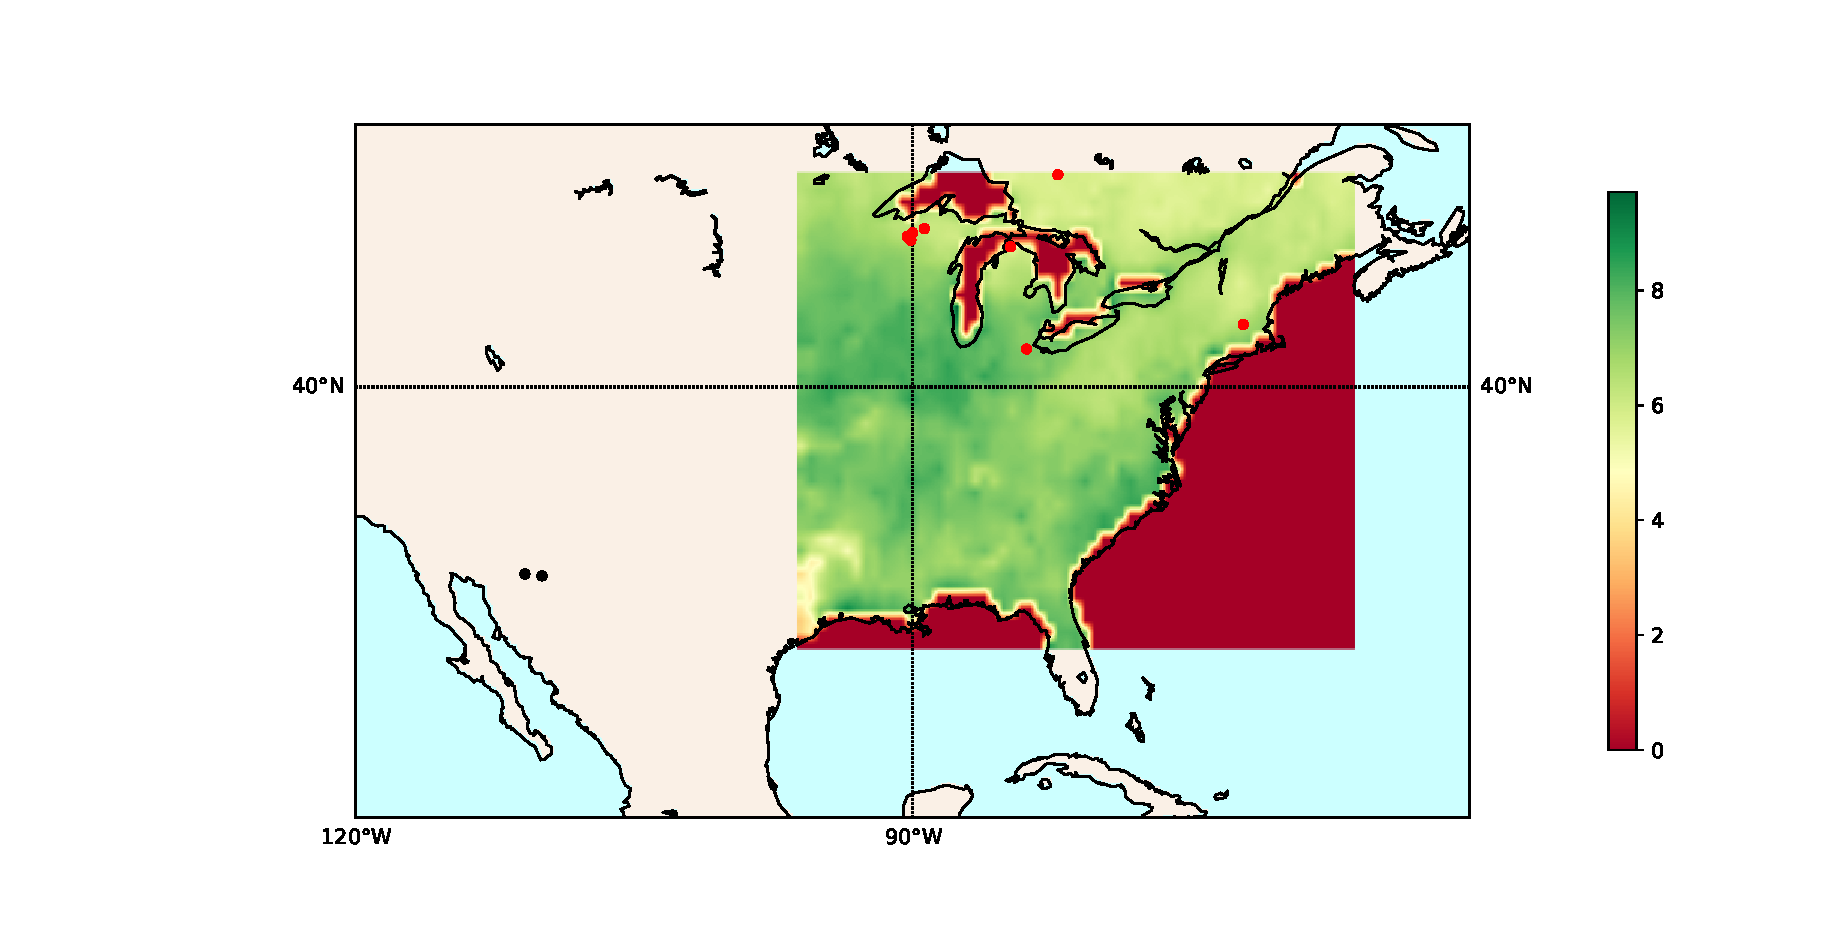
\includegraphics[width=\textwidth]{figs/map.eps}
\caption{\label{fig:map} The 8 sites that lie in the region where we have model evaluations. The average GPP field for a month of June (?) is shown.}
\end{figure}

The sensitivities for the eight sites over 12 months are shown in Figure~\ref{fig:sens} (minus the winter months with zero GPP for all ensemble members.).

\begin{figure}[!hb]
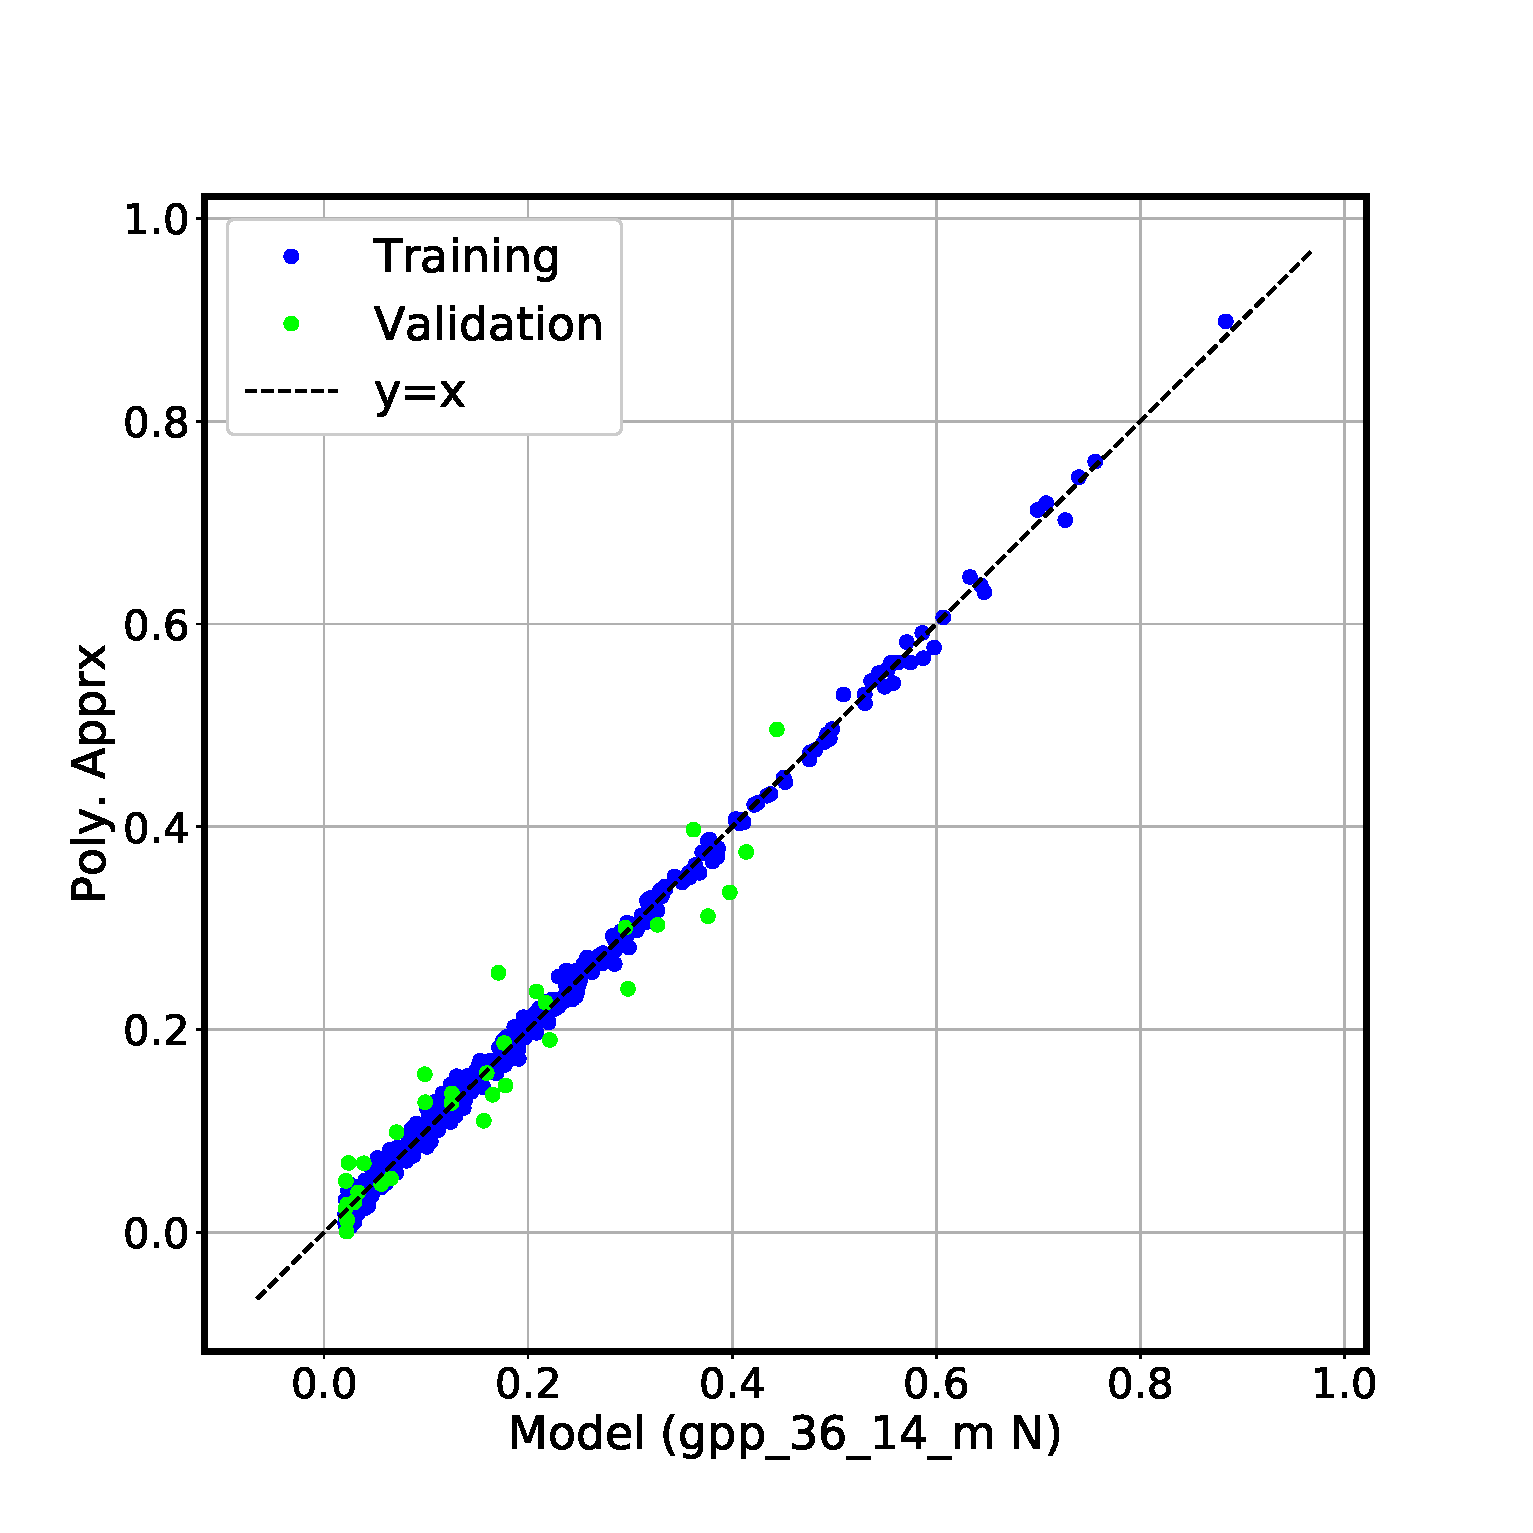
\includegraphics[width=0.53\textwidth]{figs/fit_13498.eps}\hfill
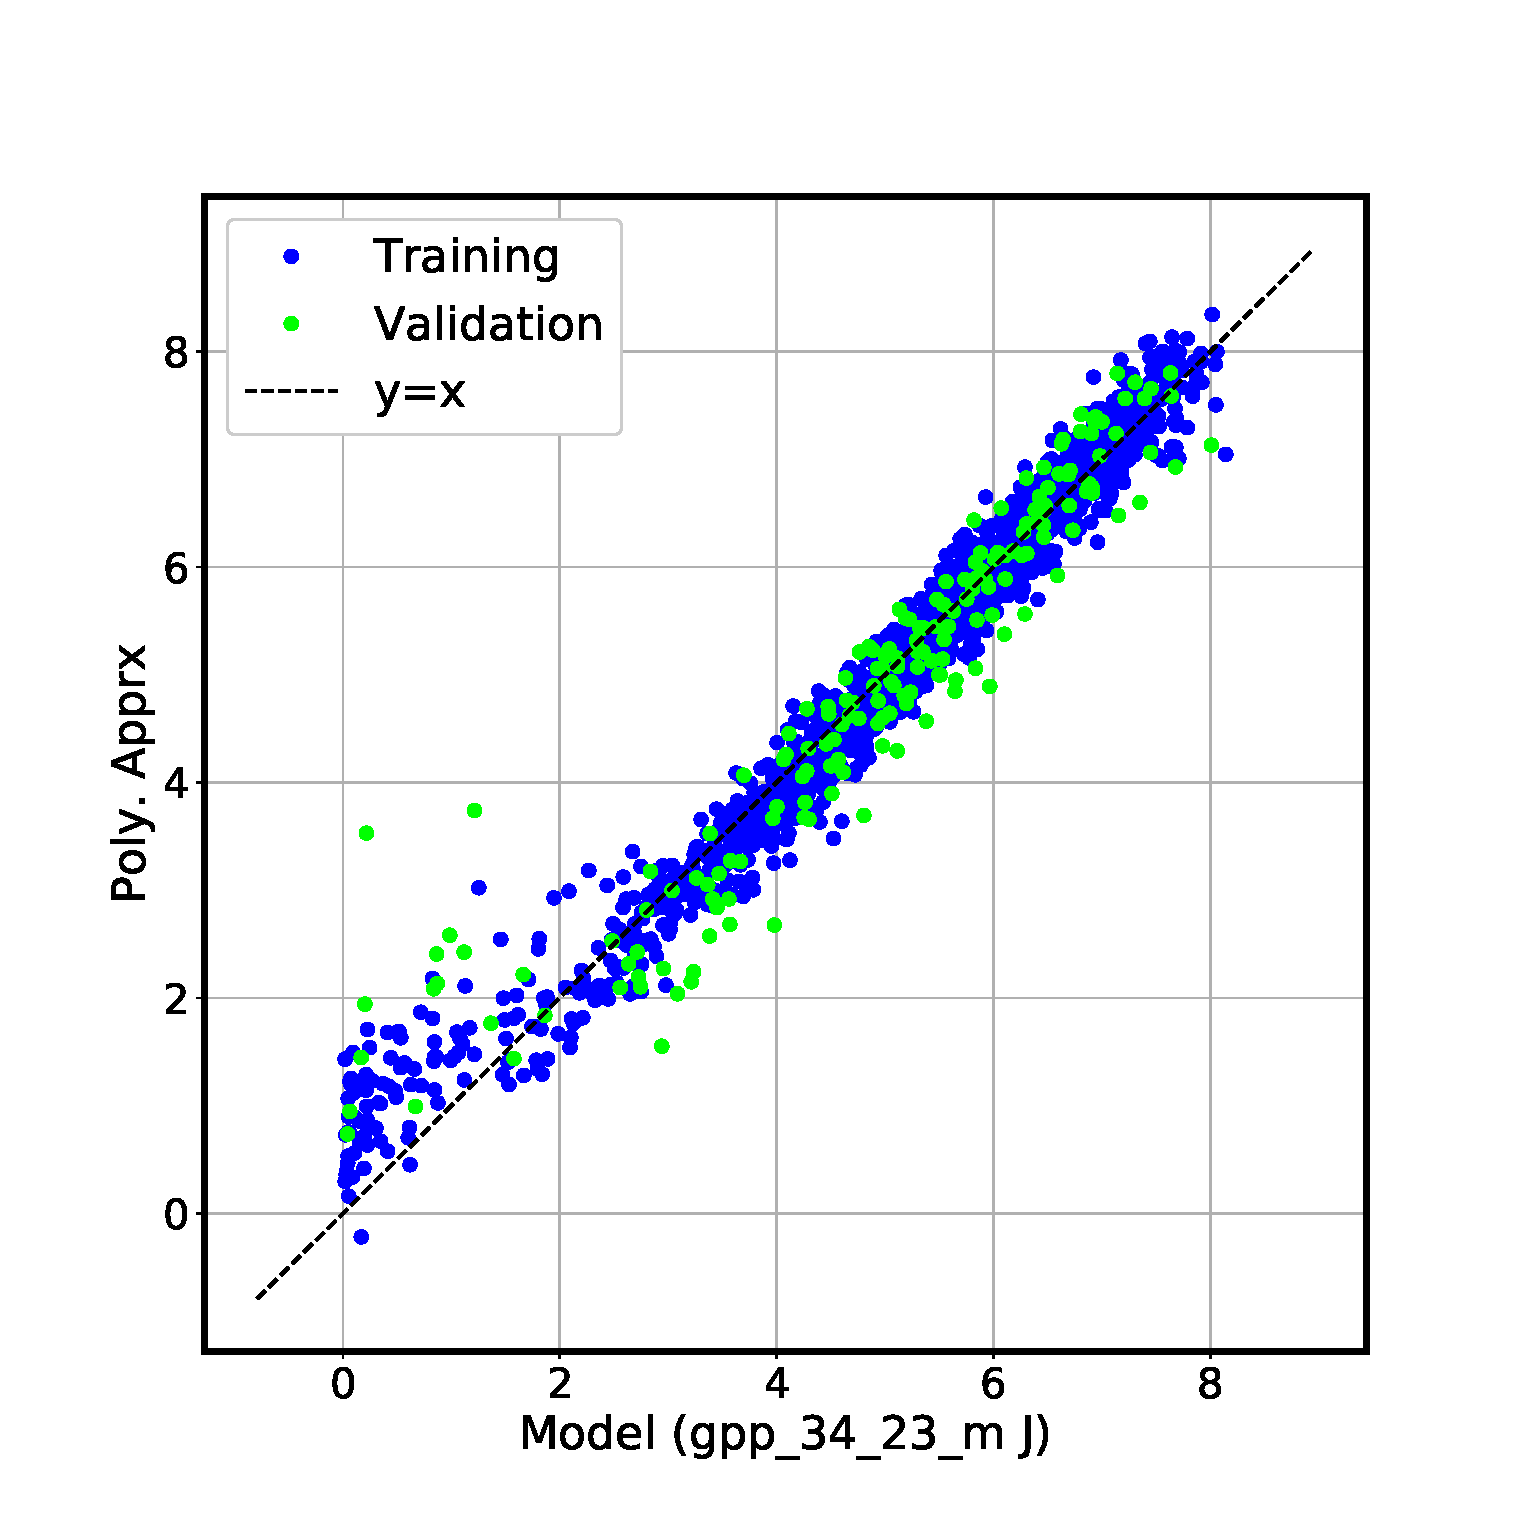
\includegraphics[width=0.53\textwidth]{figs/fit_19974.eps}
\caption{\label{fig:surr} Two representative surrogates.}
\end{figure}


\begin{figure}[!hb]
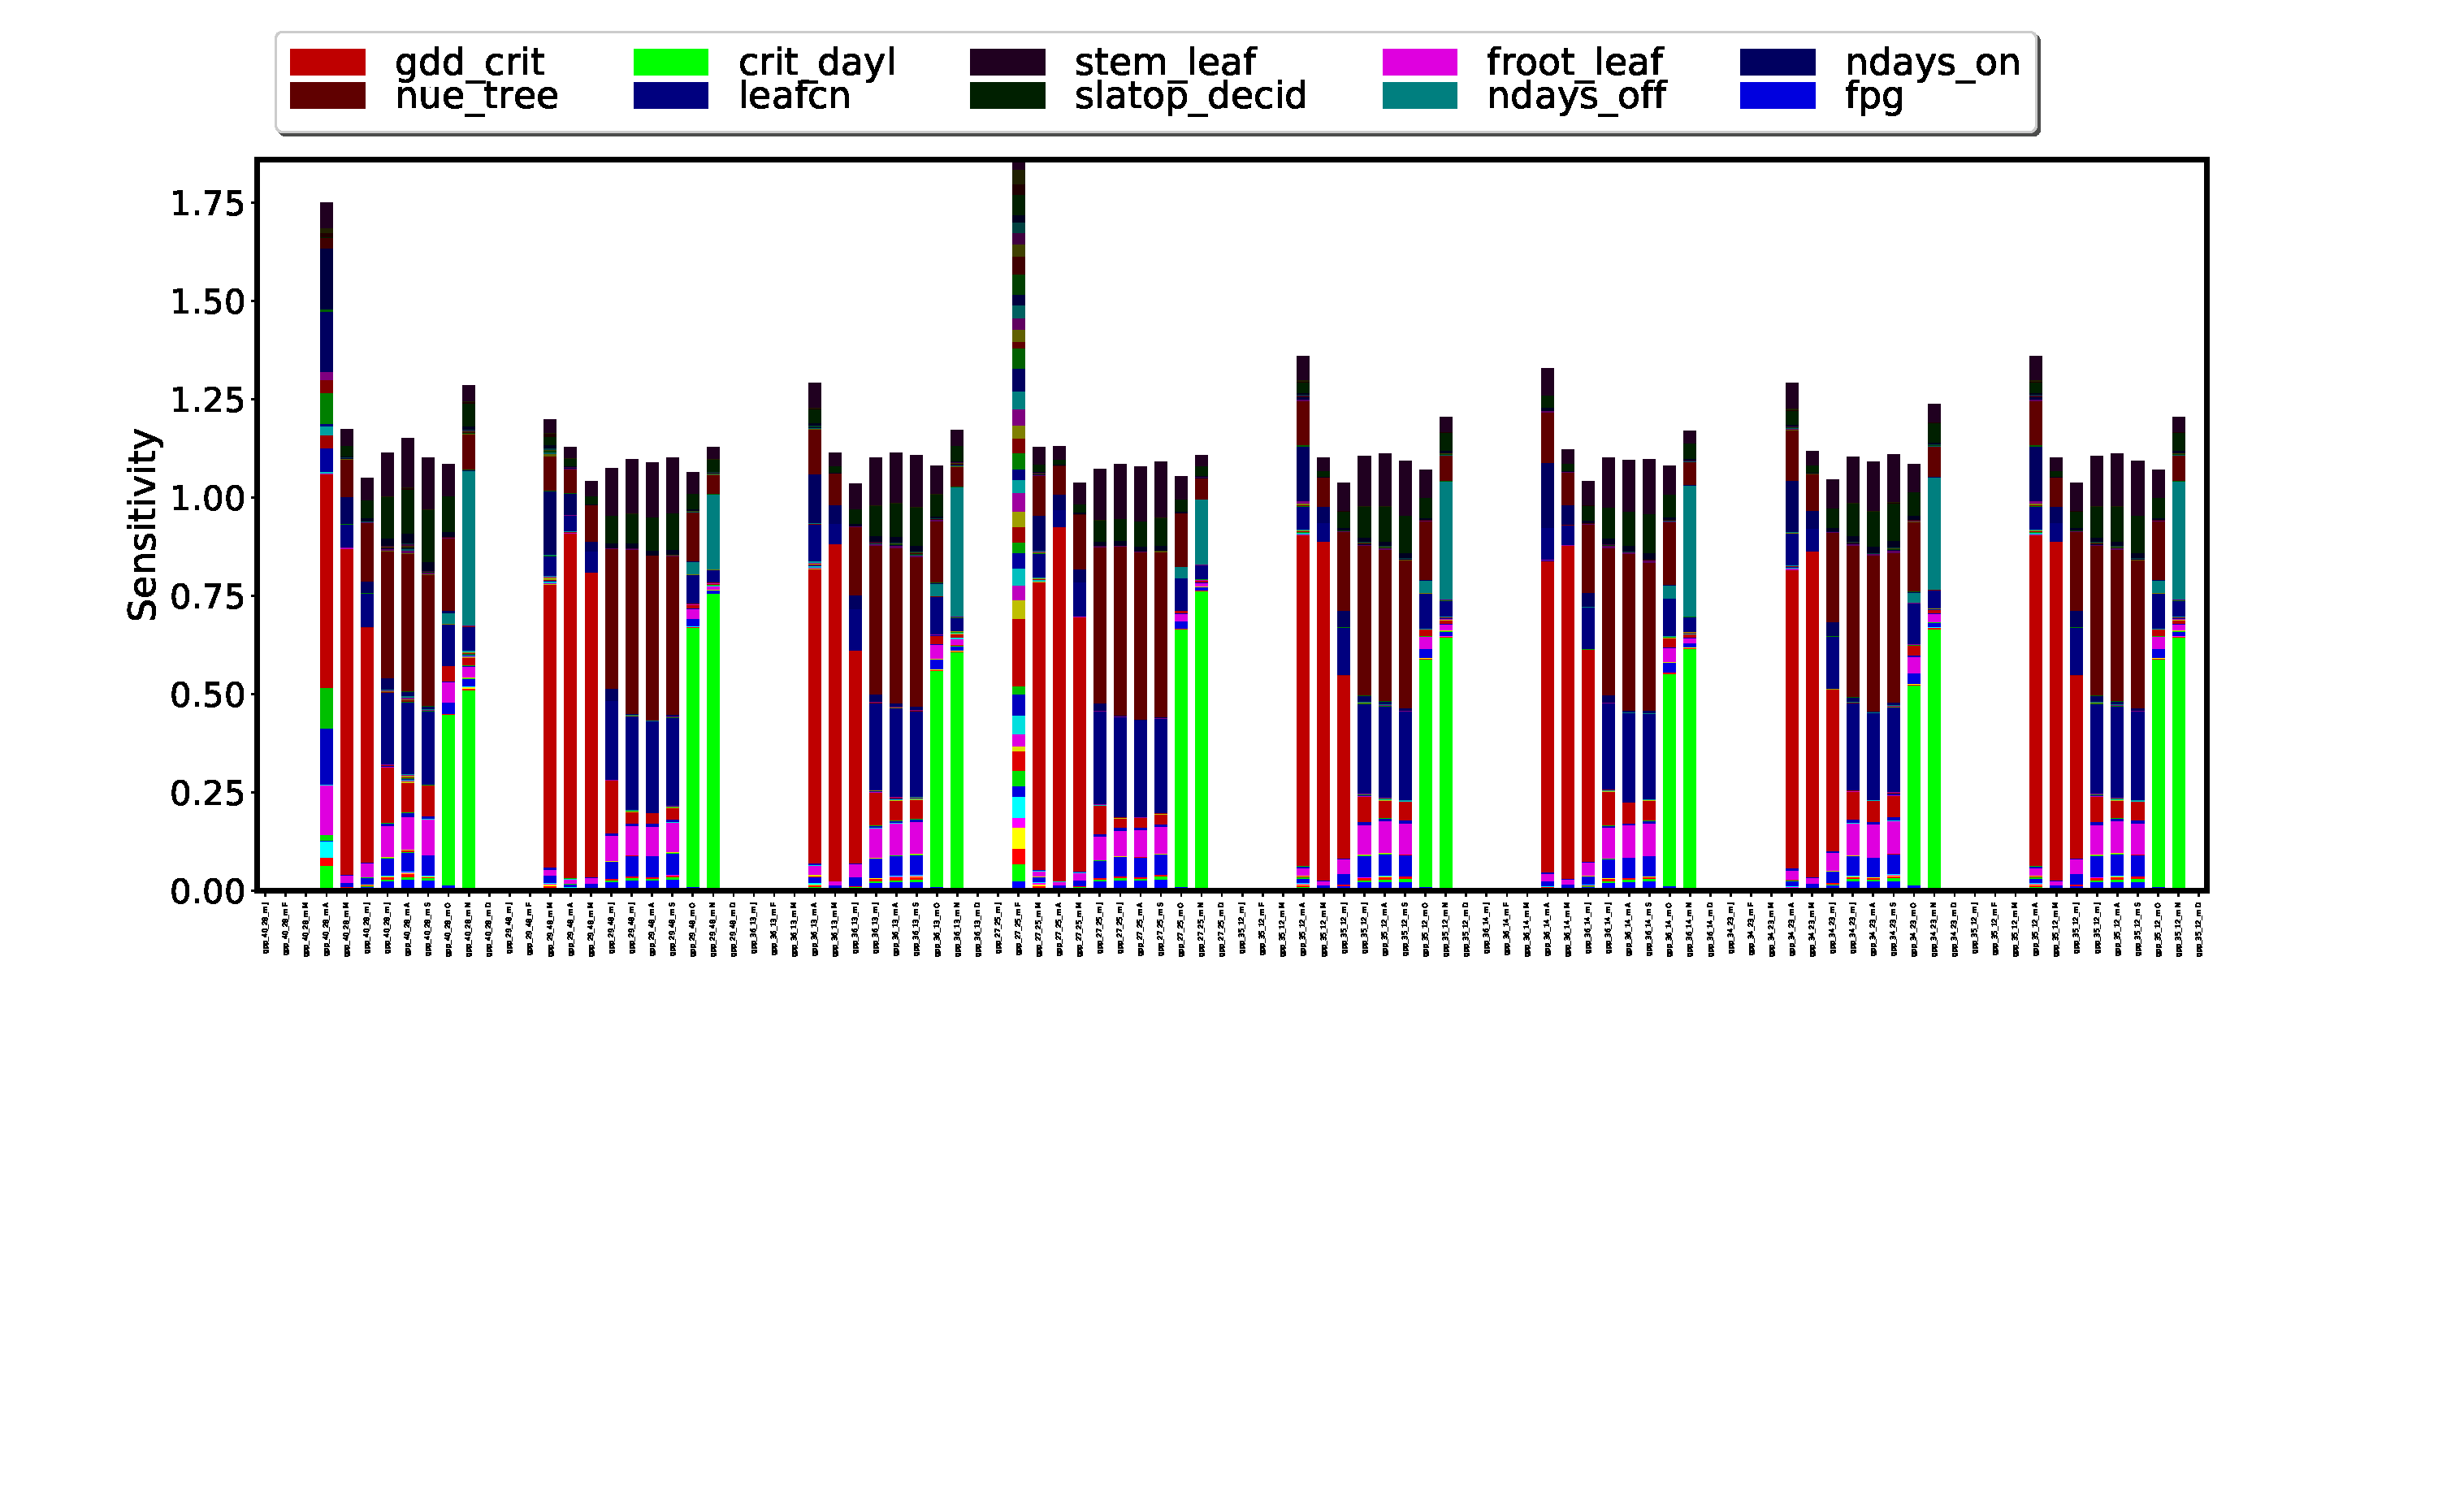
\includegraphics[width=\textwidth]{figs/sens.eps}
\caption{\label{fig:sens} Sensitivities of GPP for 8 sites (the winter sites are not shown due to dominantly zero-ed GPP). }
\end{figure}

\section{Data}

Similarly, we have observational daily data for $S=8$ sites that is averaged to obtain monthly data before averaging over years to obtain month-by-month data - a total of $12S=96$ data points $\{h_{ij}\}$ for $i=1,\dots,S$ and $j=1,\dots 12$.

\section{Inference}

\subsection{Classical}
The classical surrogate-enabled inference setup: iid Gaussian noise on $h_{ij}-Q^c_{ij}(\lambda)$. [More details to write later]. We selected the top four most sensitive parameters
\verb#gdd_crit, nue_tree, crit_dayl, leafcn# for inference. See Figures~\ref{fig:fits1} and~\ref{fig:fits2} for the posterior predictive. [MCMC and parameter posteriors to come later]

\subsection{Model error}
[to come later as need arises.]


\begin{figure}[!hb]
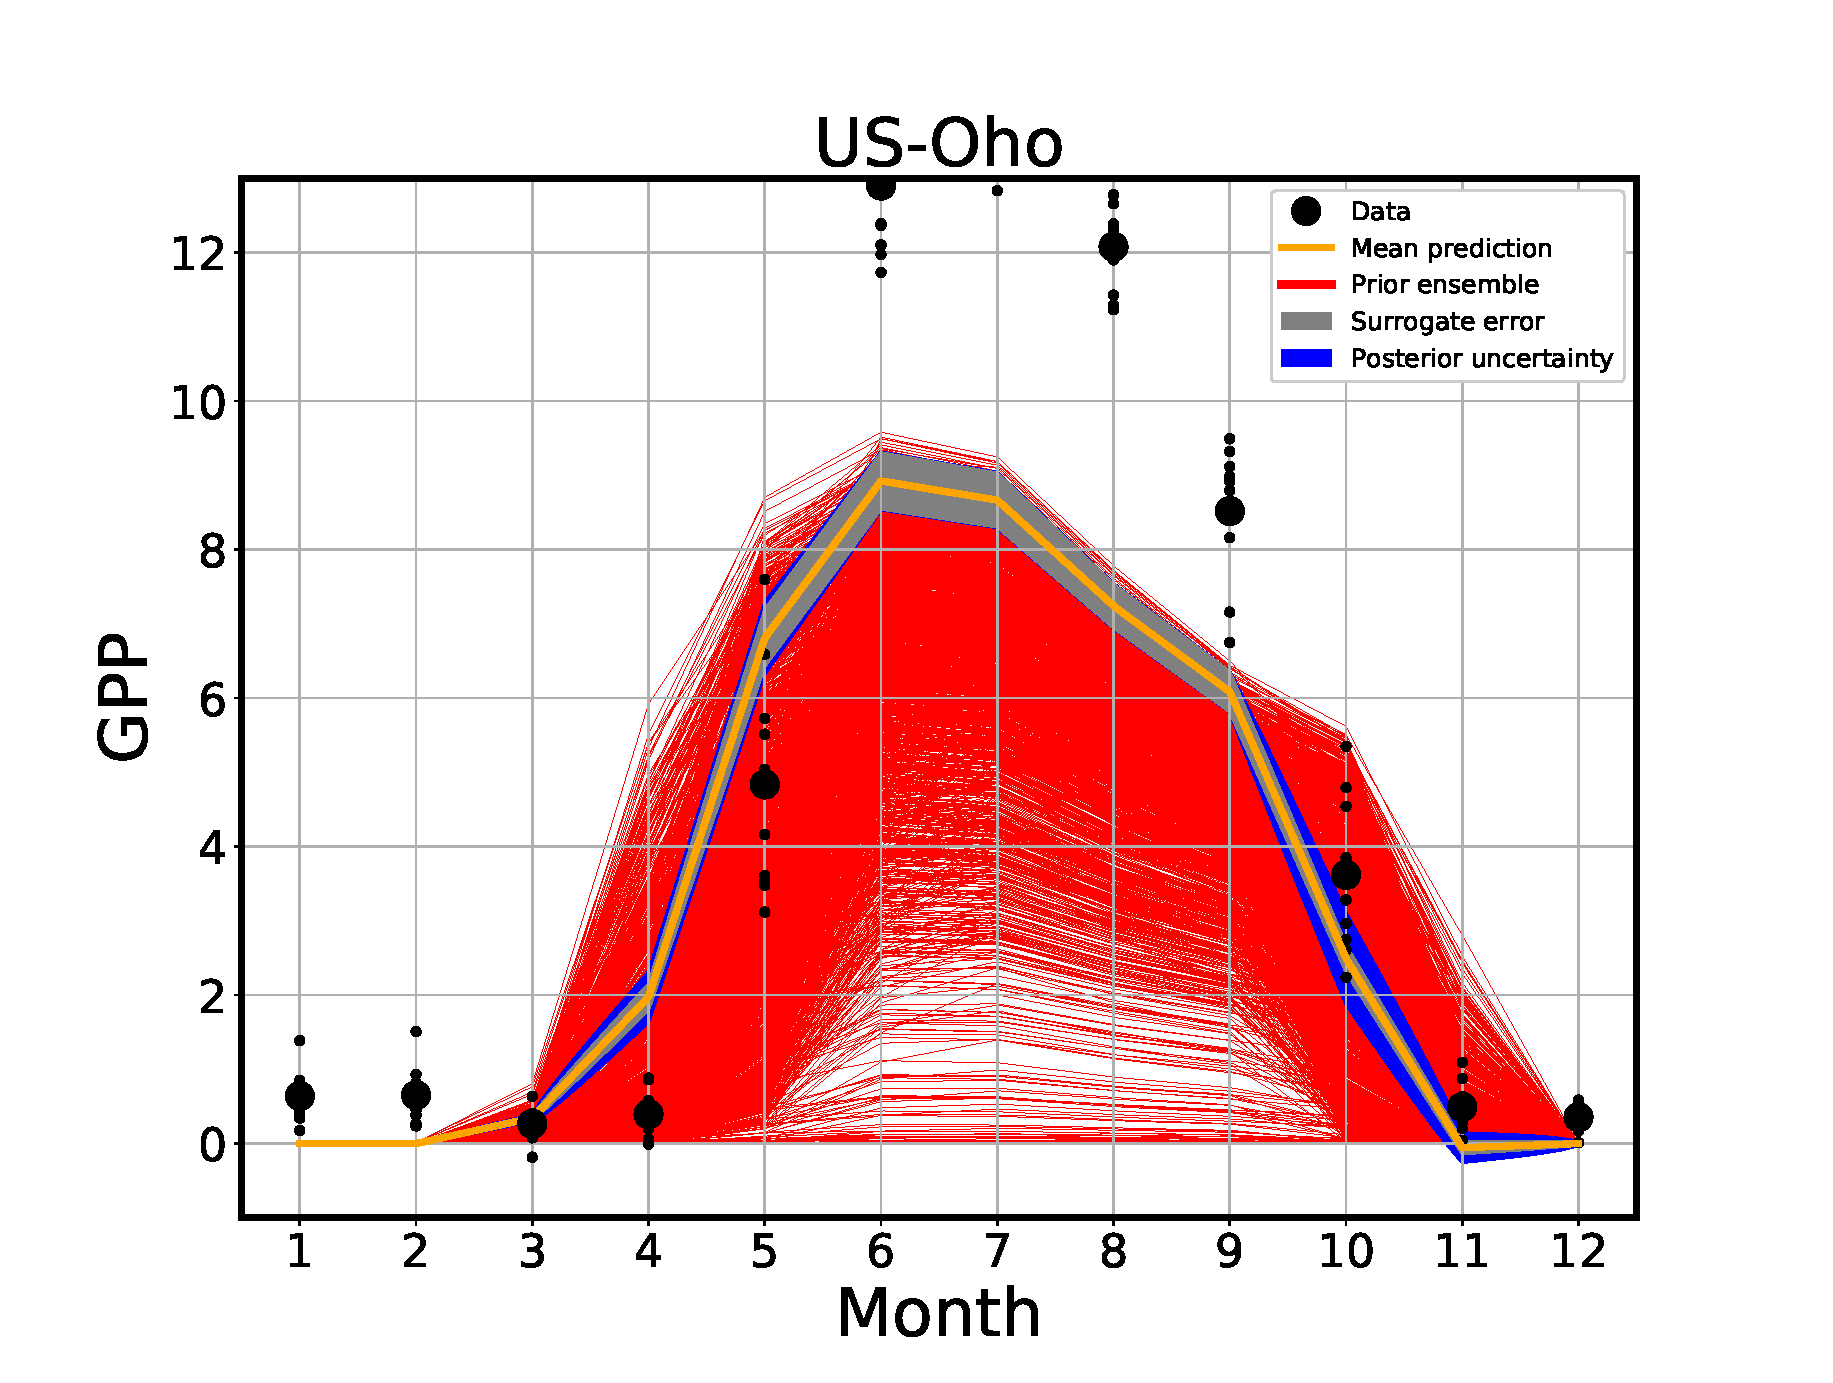
\includegraphics[width=0.53\textwidth]{figs/fit1d_27_25.eps}\hfill
\includegraphics[width=0.53\textwidth]{figs/fitshade_27_25.eps}\\
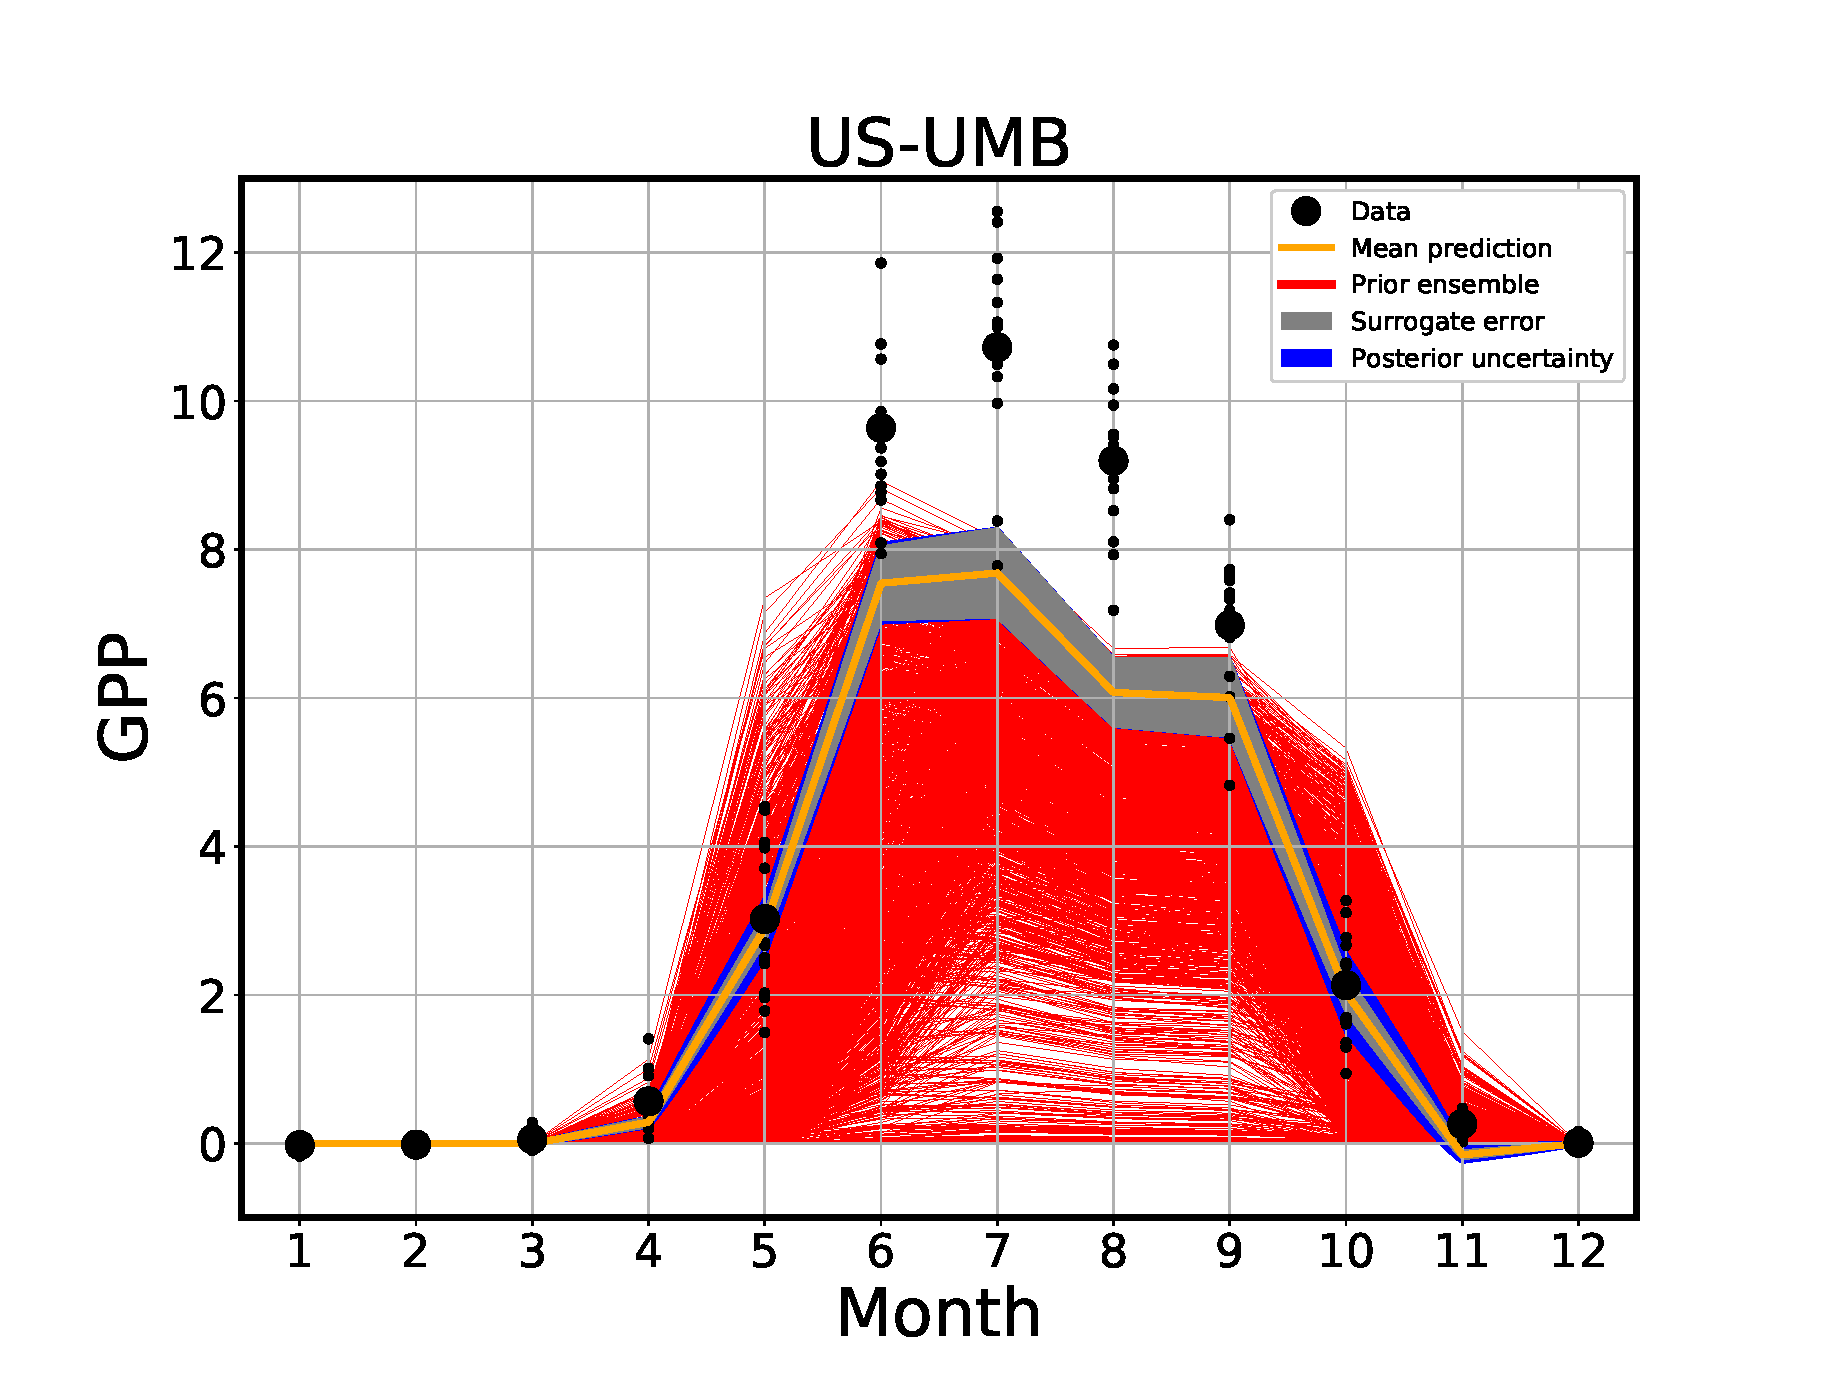
\includegraphics[width=0.53\textwidth]{figs/fit1d_34_23.eps}\hfill
\includegraphics[width=0.53\textwidth]{figs/fitshade_34_23.eps}\\
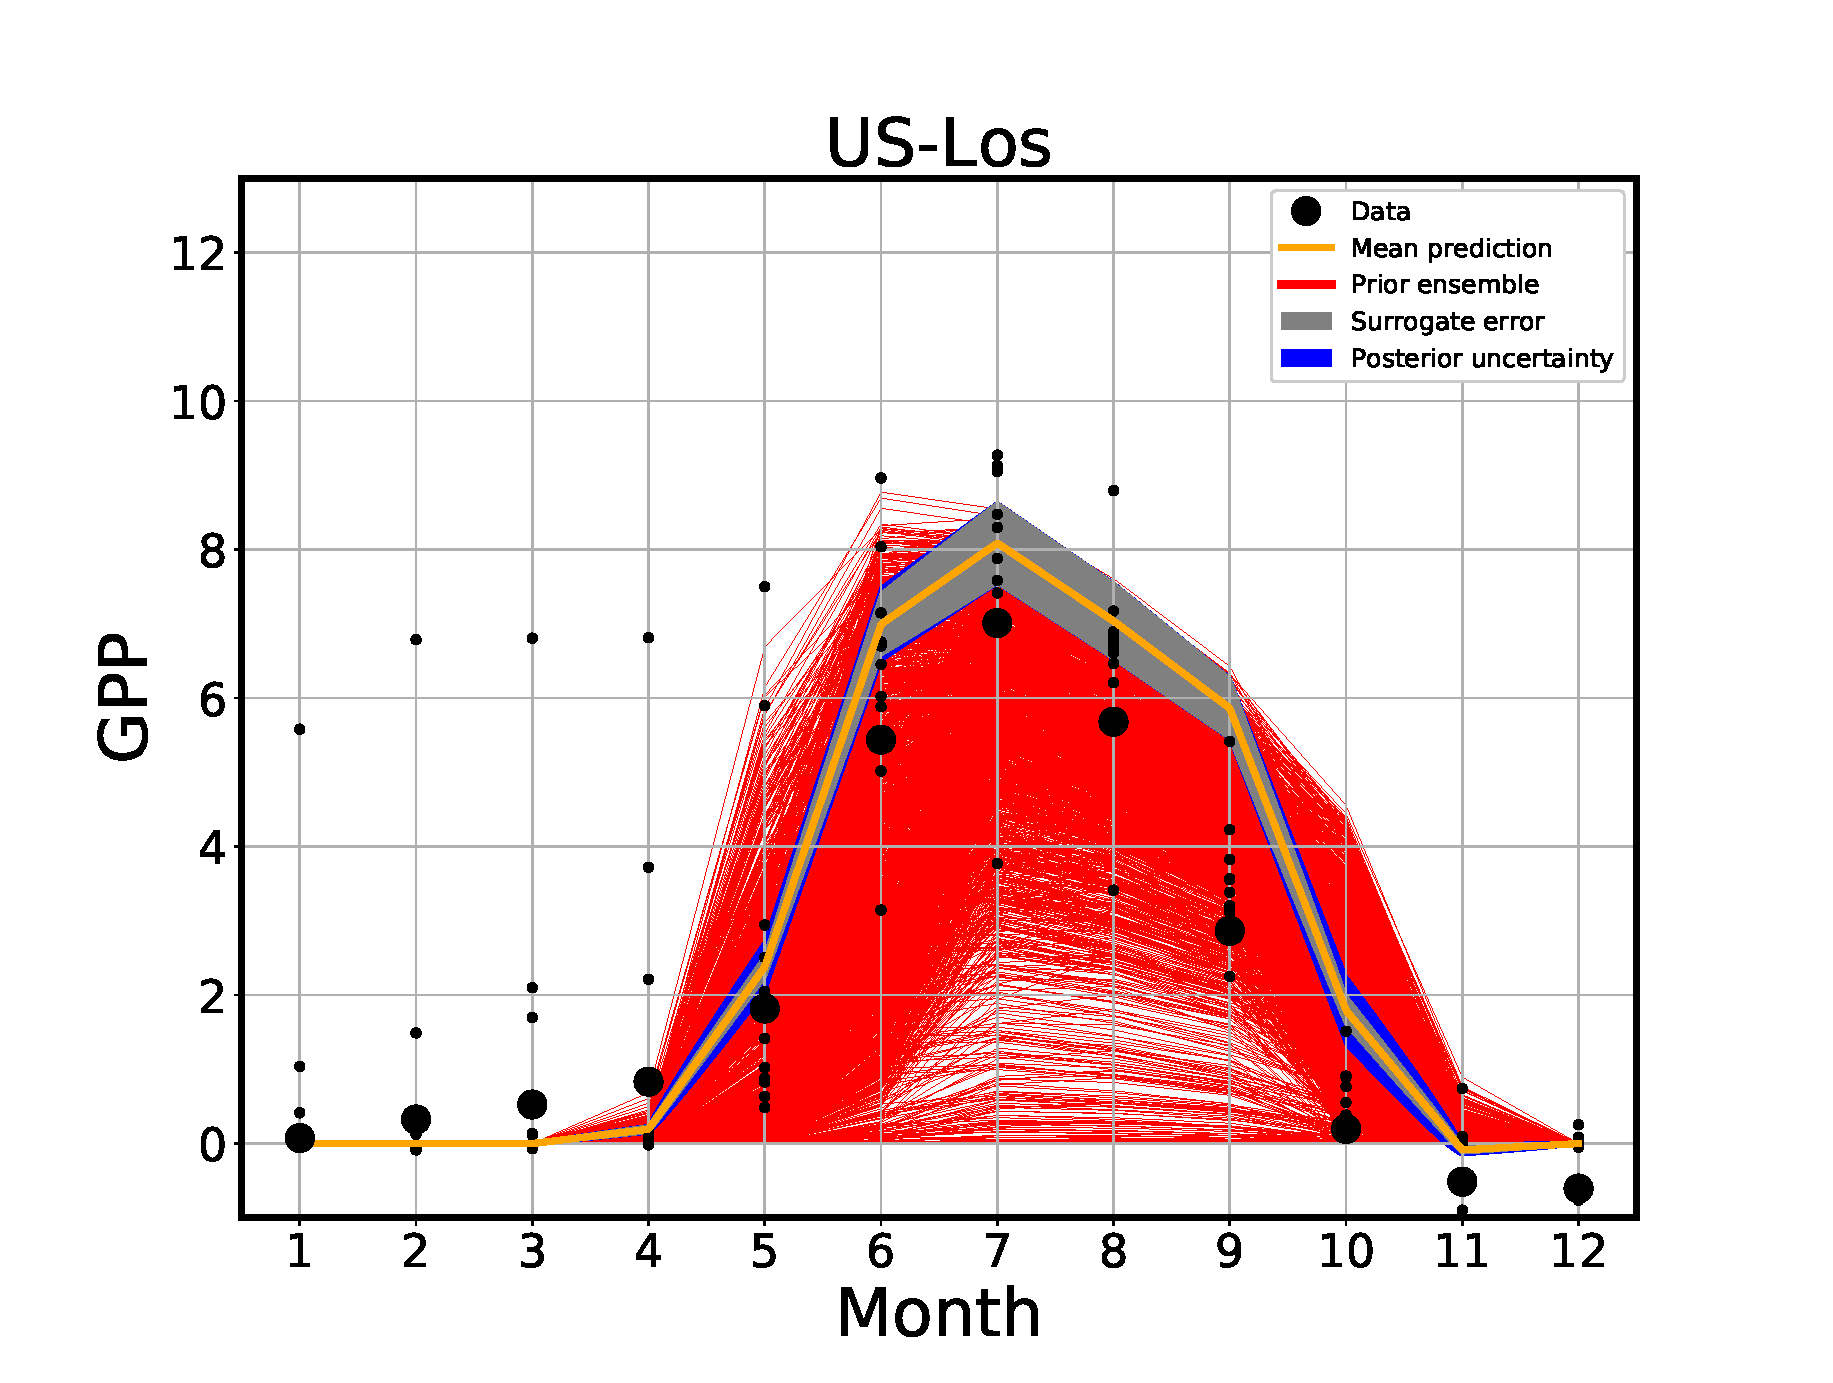
\includegraphics[width=0.53\textwidth]{figs/fit1d_36_13.eps}\hfill
\includegraphics[width=0.53\textwidth]{figs/fitshade_36_13.eps}
\caption{\label{fig:fits1} Inference1. Large black dots are the mean data points, smaller ones are all samples across years. The right column, the shaded plots, show prior (red) and posterior (green) quantiles.}
\end{figure}
\begin{figure}[!hb]
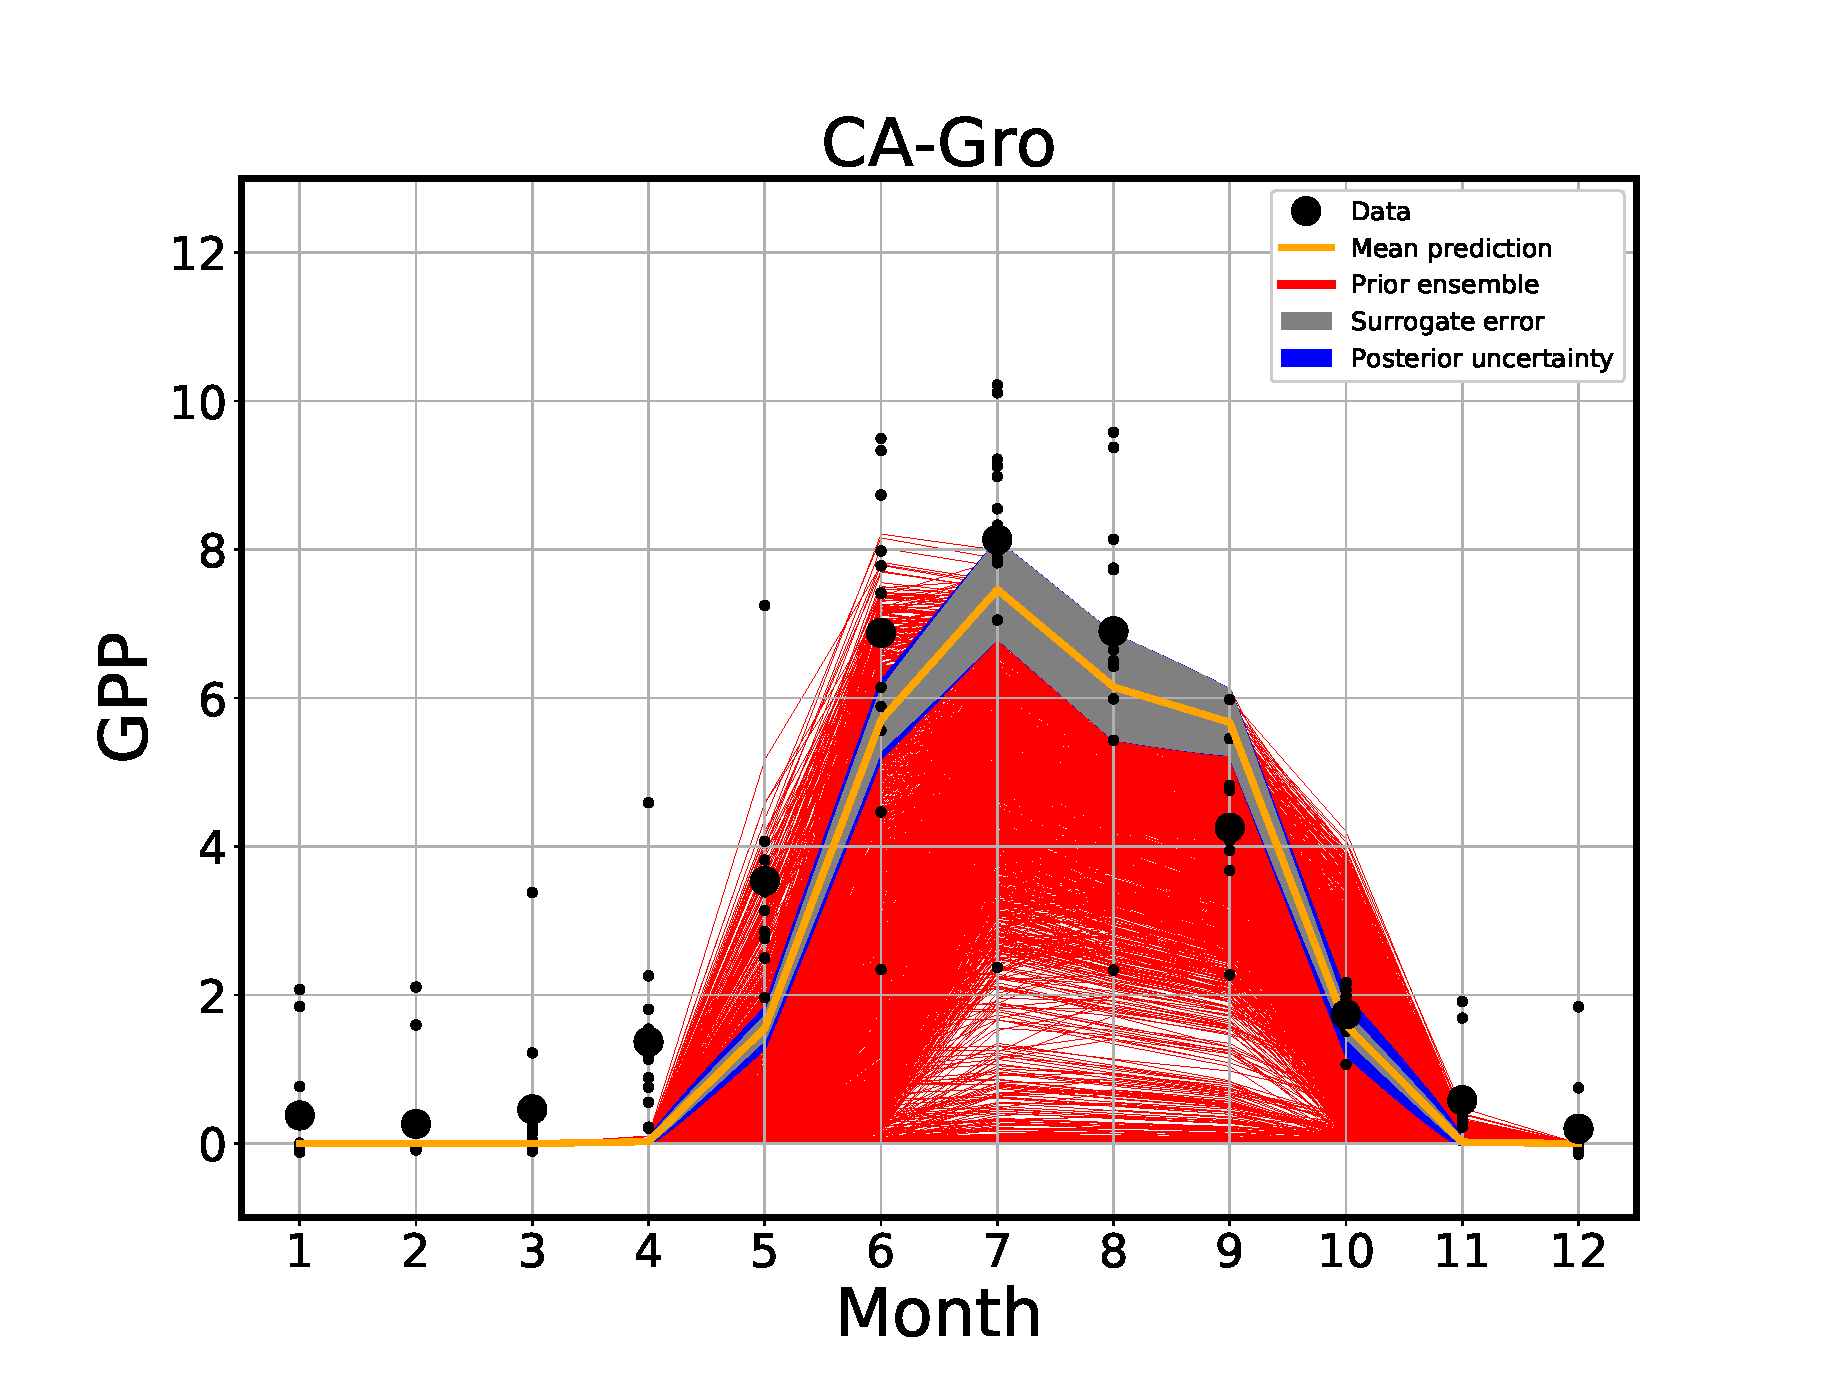
\includegraphics[width=0.53\textwidth]{figs/fit1d_40_28.eps}\hfill
\includegraphics[width=0.53\textwidth]{figs/fitshade_40_28.eps}\\
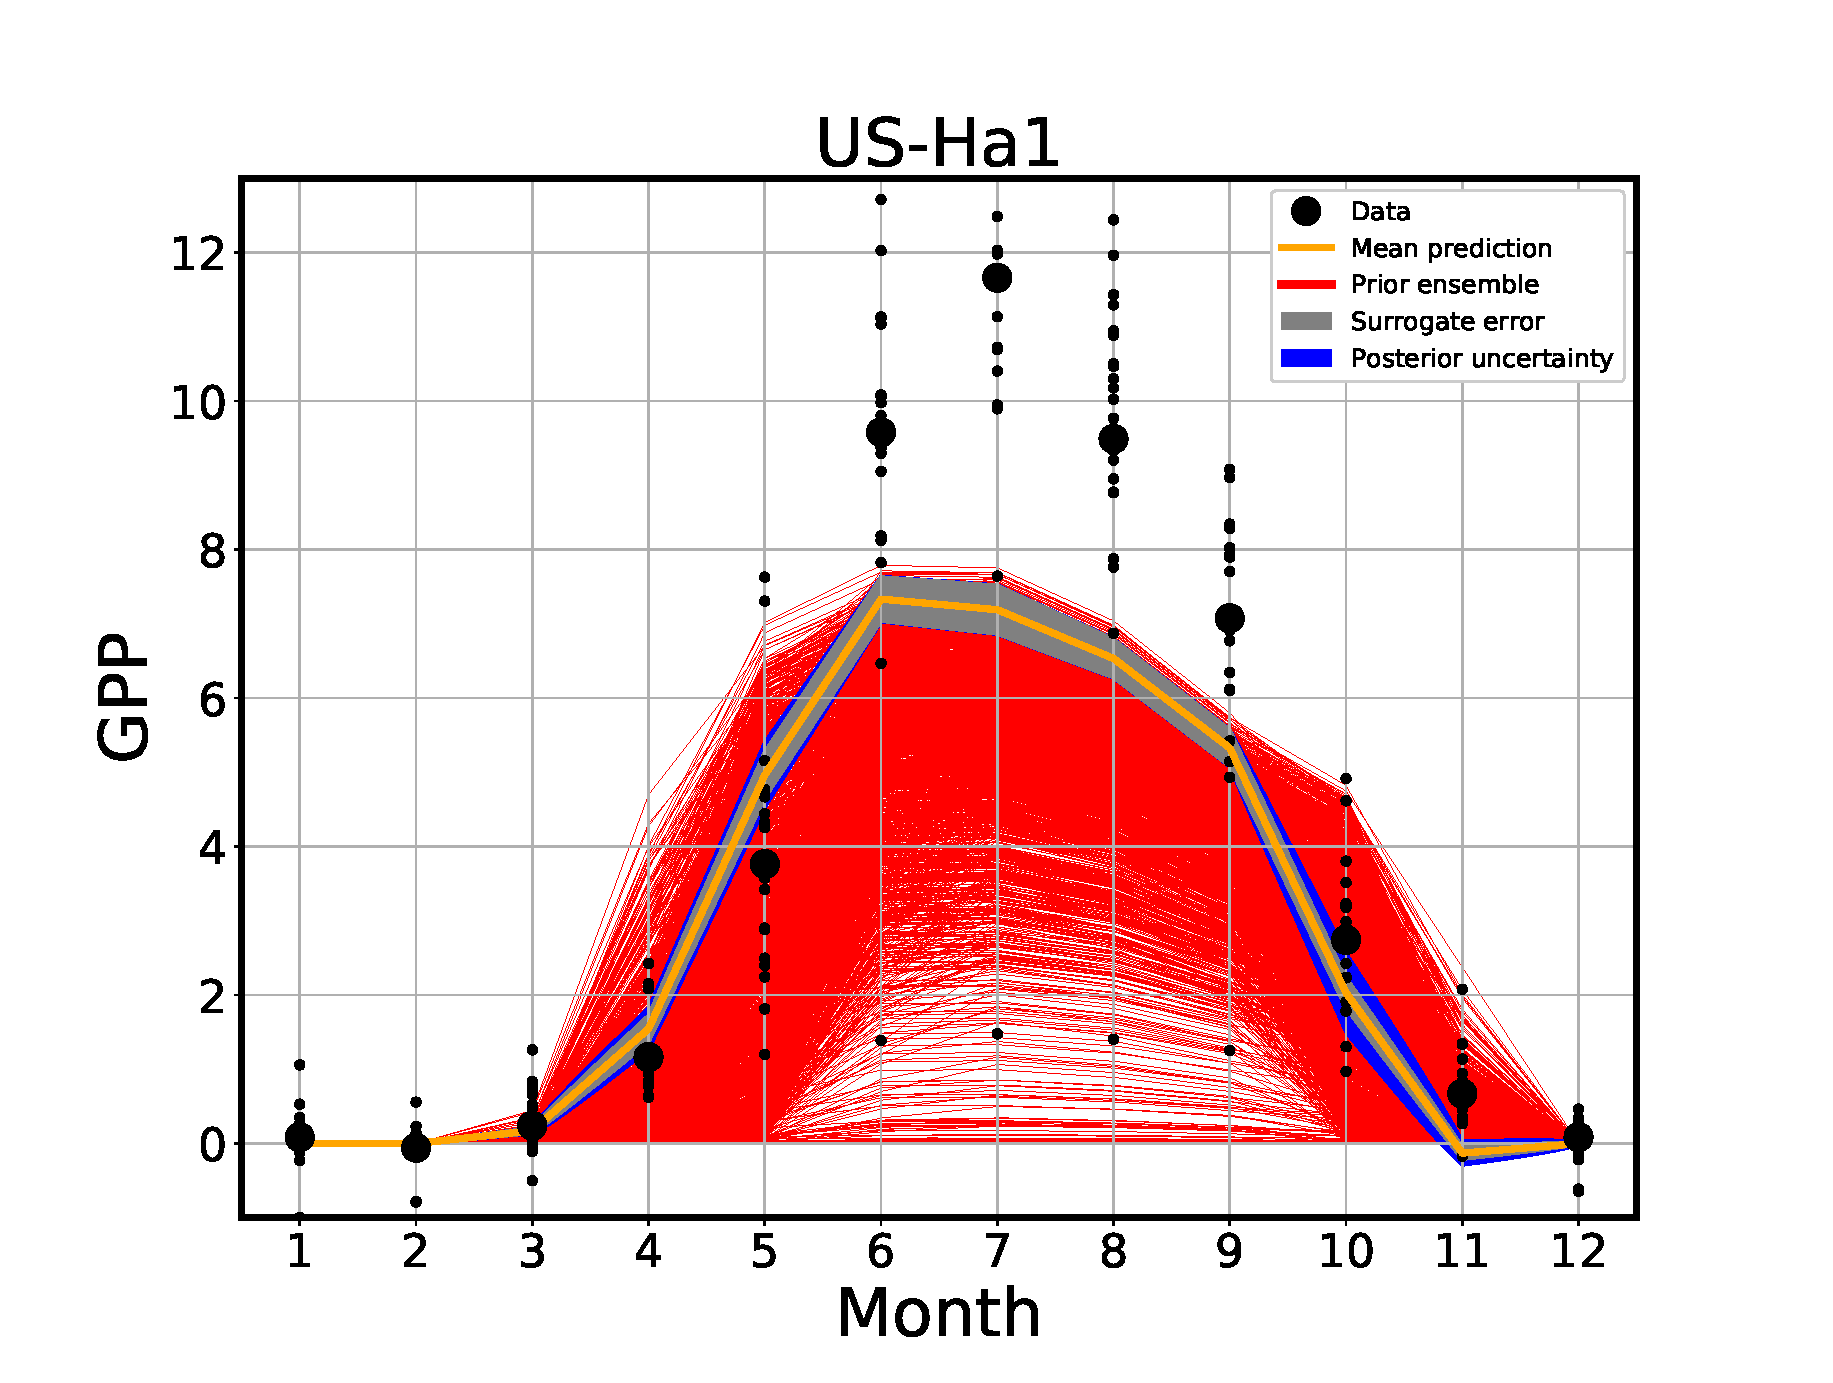
\includegraphics[width=0.53\textwidth]{figs/fit1d_29_48.eps}\hfill
\includegraphics[width=0.53\textwidth]{figs/fitshade_29_48.eps}\\
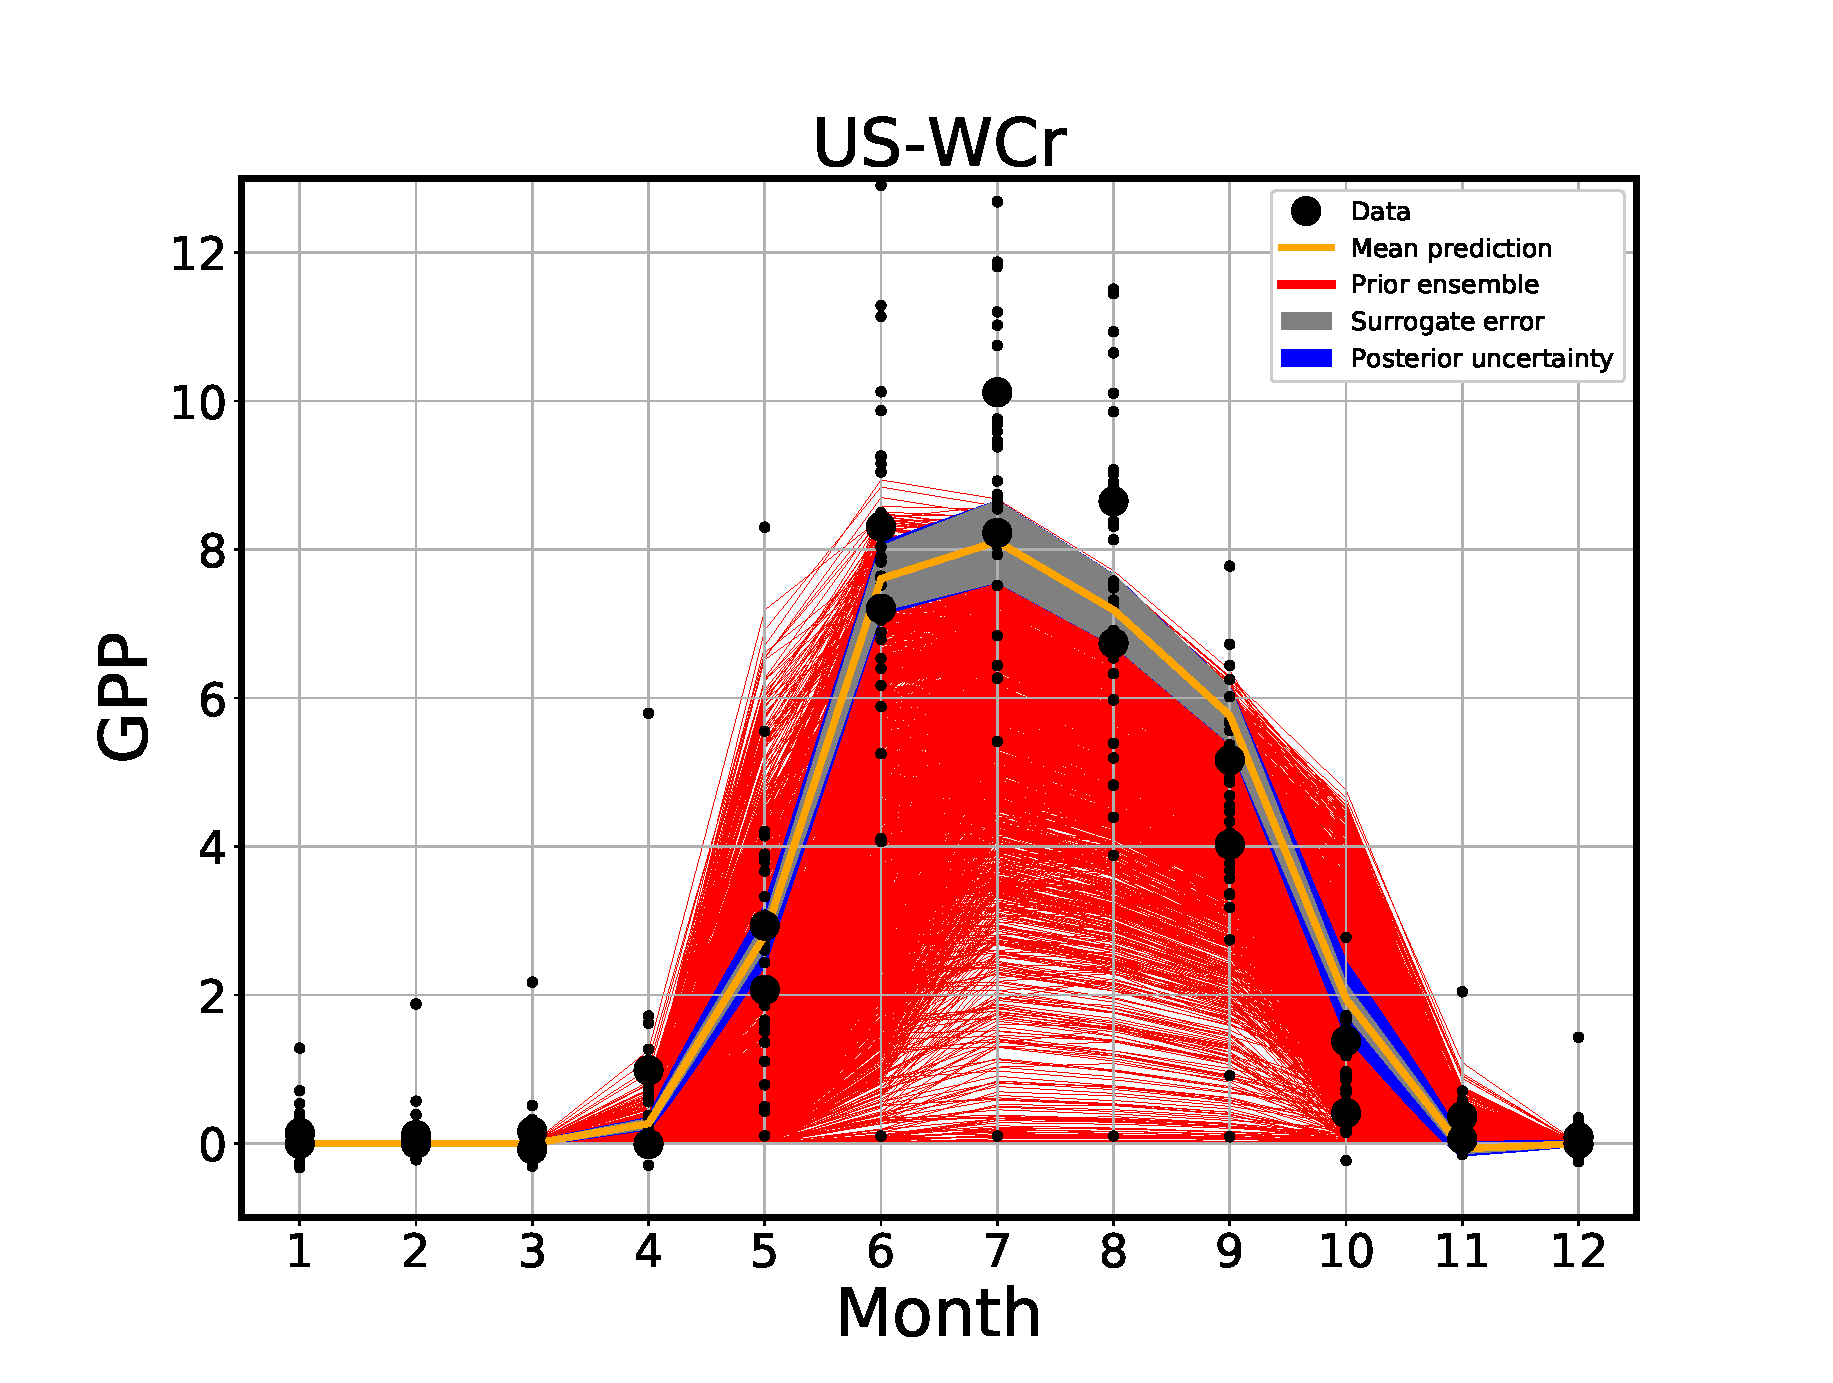
\includegraphics[width=0.53\textwidth]{figs/fit1d_35_12.eps}\hfill
\includegraphics[width=0.53\textwidth]{figs/fitshade_35_12.eps}\\
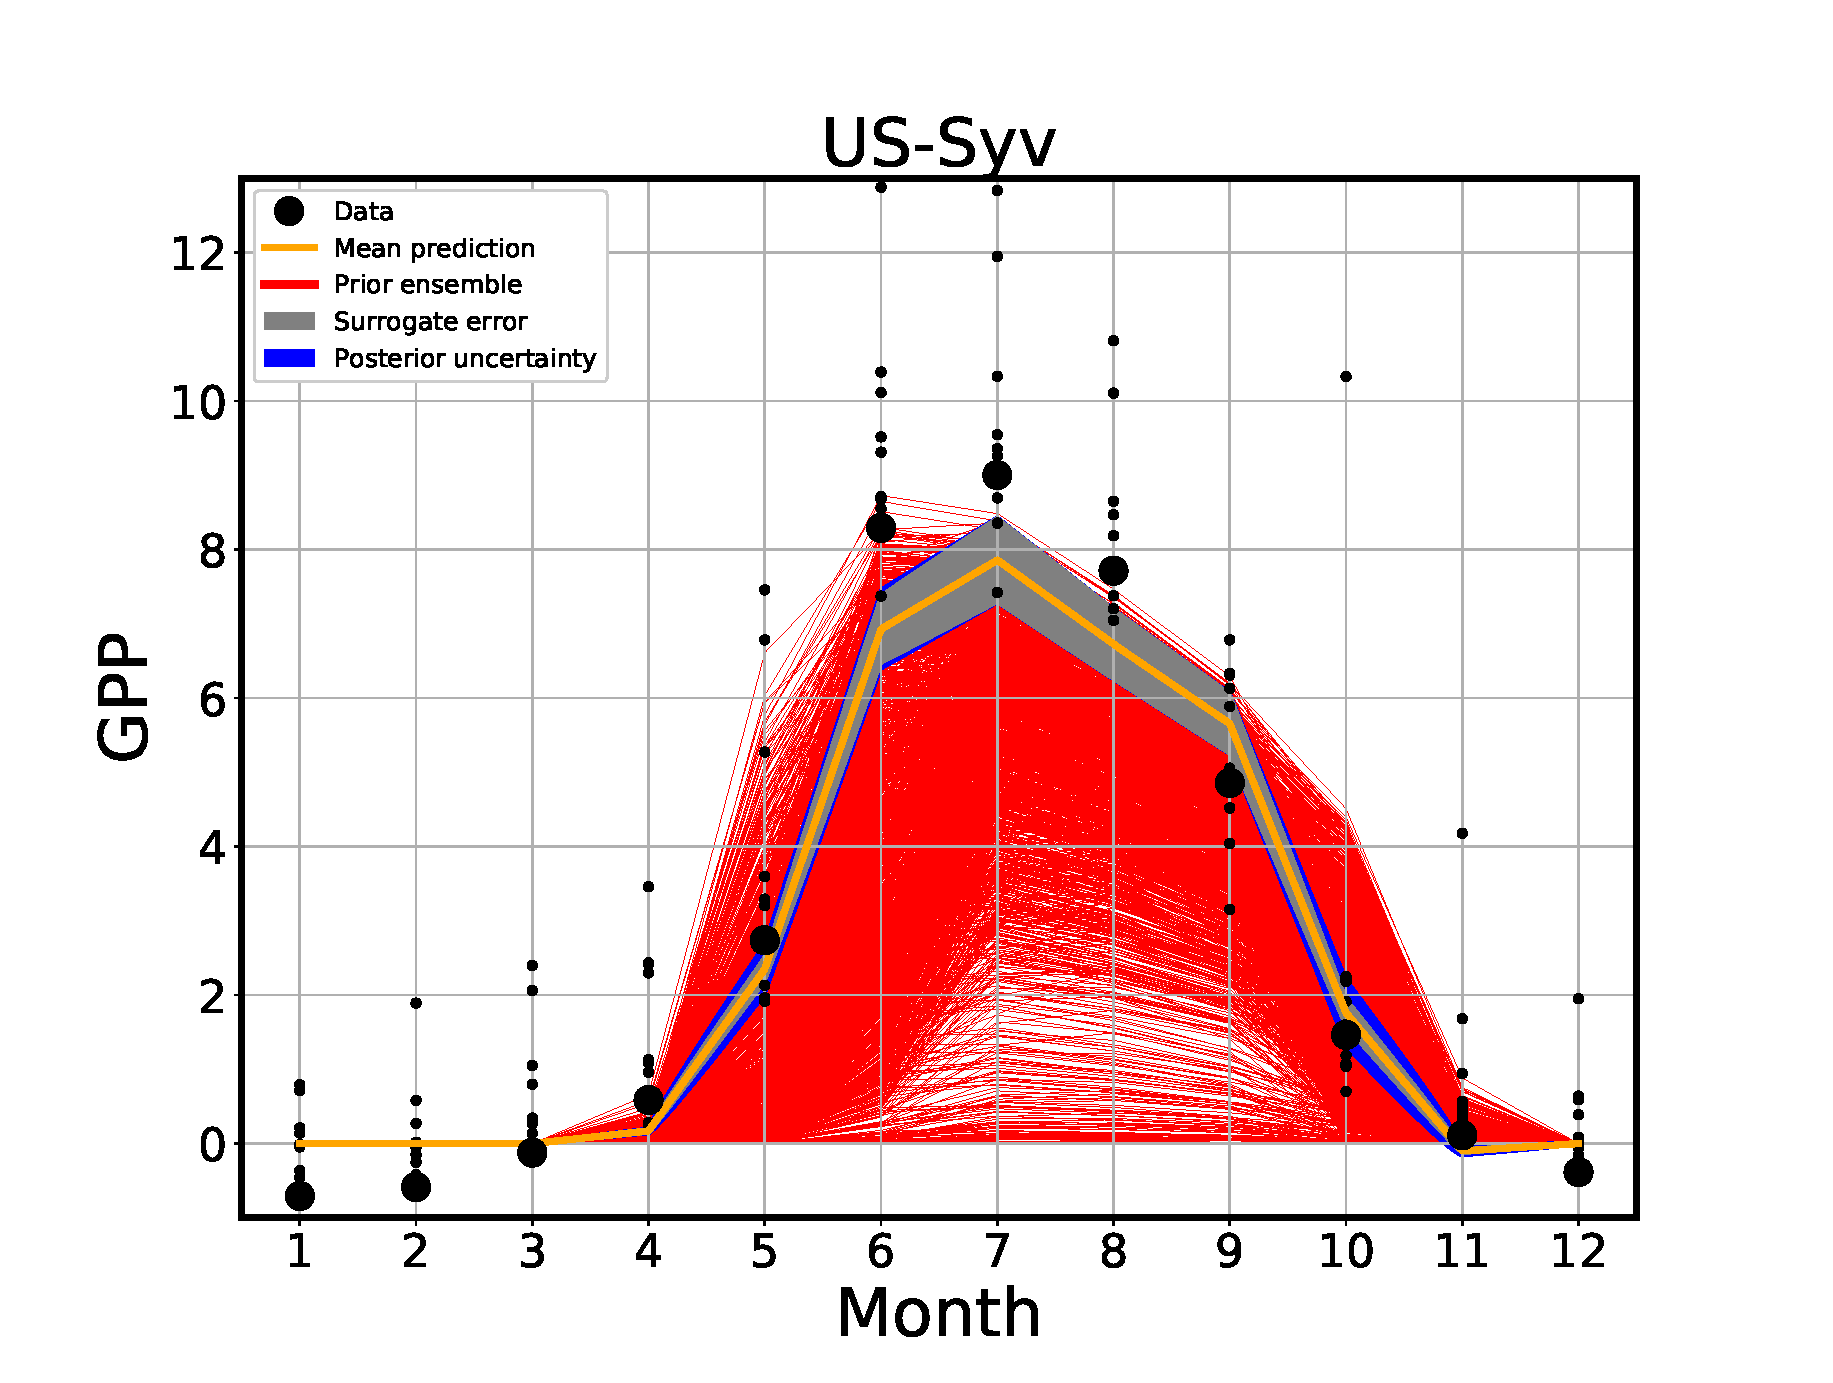
\includegraphics[width=0.53\textwidth]{figs/fit1d_36_14.eps}\hfill
\includegraphics[width=0.53\textwidth]{figs/fitshade_36_14.eps}
\caption{\label{fig:fits2} Inference2. (US-WCr includes data from US-PFa as well - they both match with the same cell in the regional simulation.)}
\end{figure}

\section{Dimensionality reduction via Karhunen-Lo{\`e}ve expansions}
 [ongoing] [will add technical details later]. Plots of mean field and eigenvalue decay are in Figure~\ref{fig:kl}.


\begin{figure}[!hb]
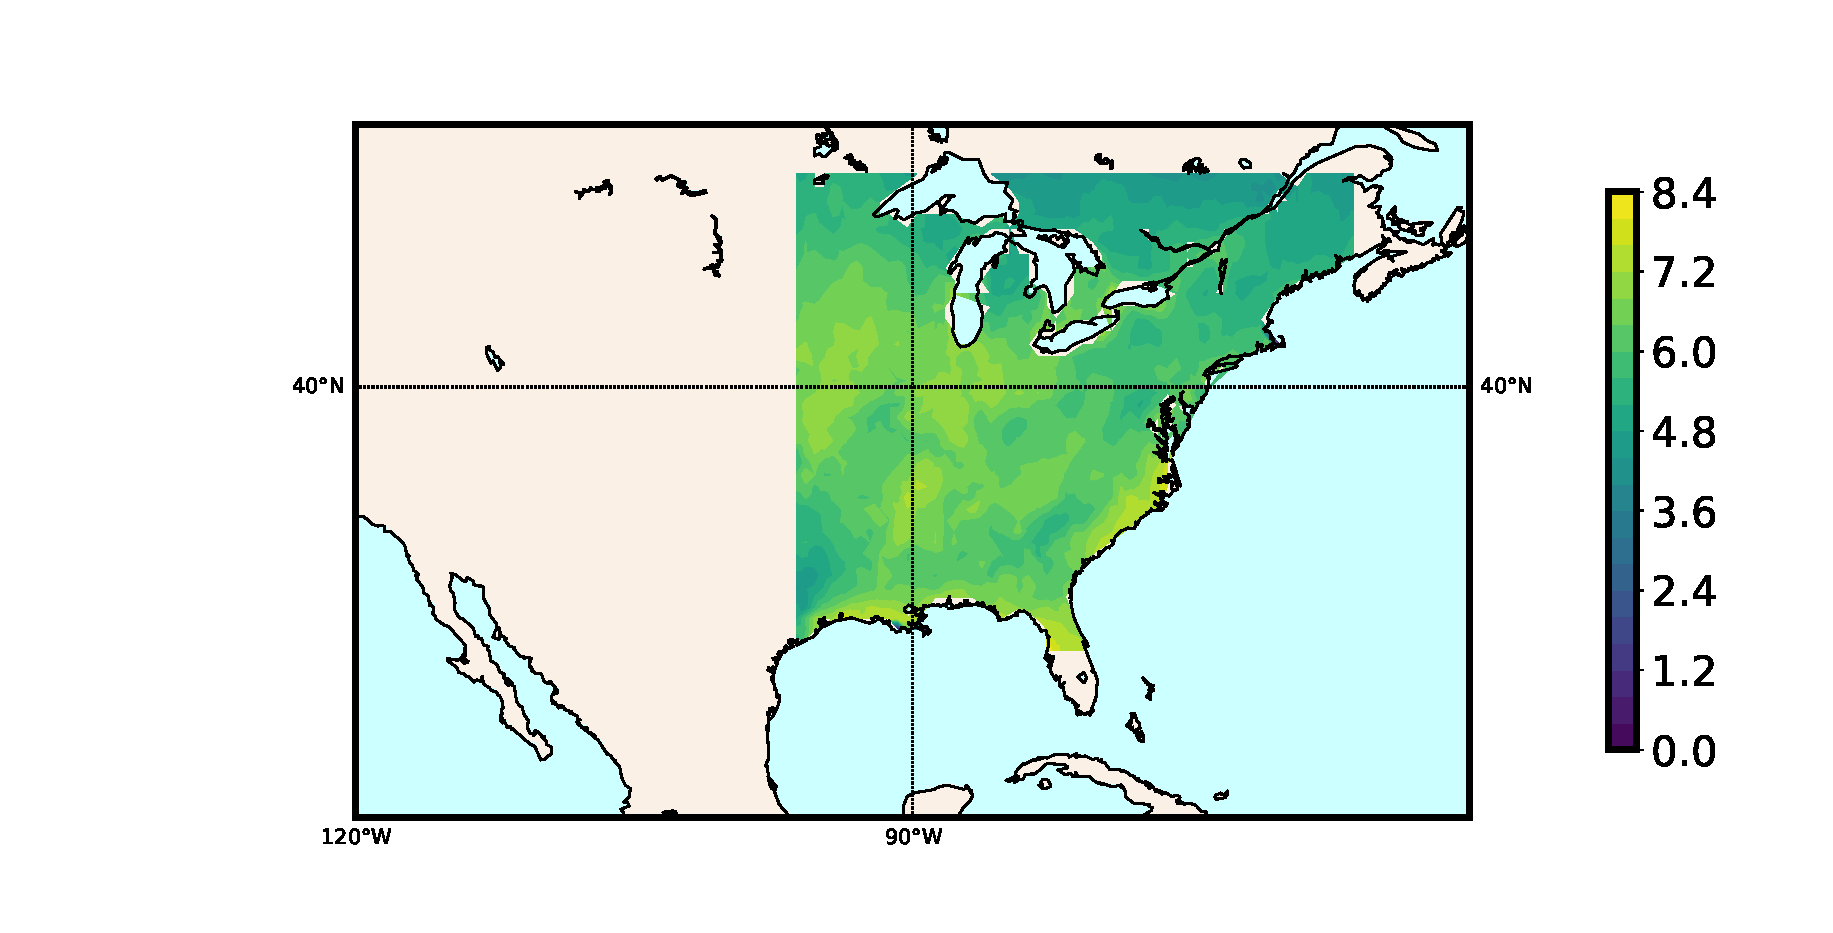
\includegraphics[height=0.33\textwidth]{figs/map_mean_kl.eps}\hfill
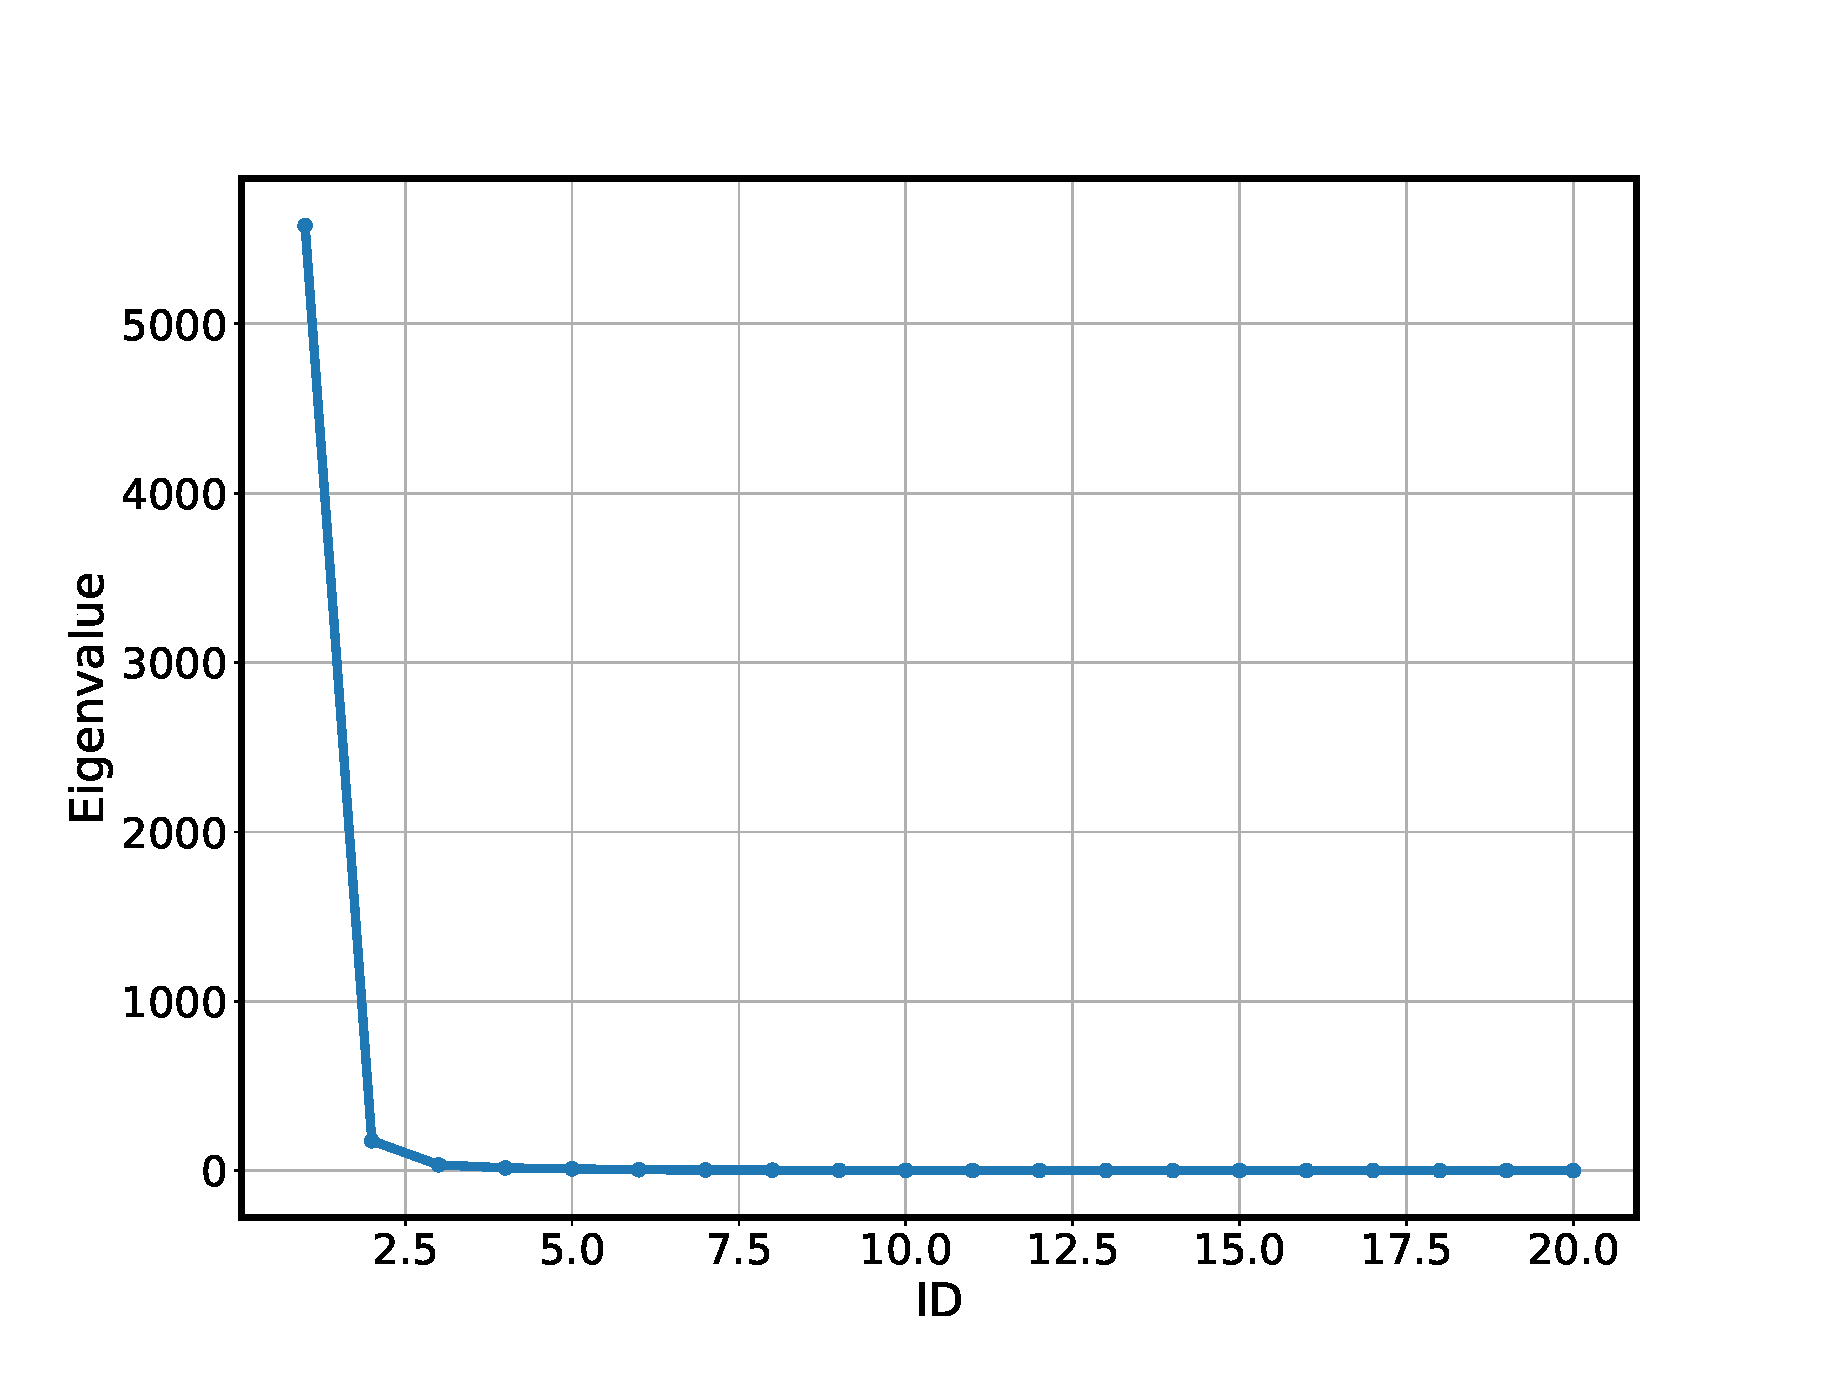
\includegraphics[height=0.33\textwidth]{figs/eig.eps}
\caption{\label{fig:kl} Mean KL field and eigenvalue decay.}
\end{figure}



%%%%%%%%%%%%%%%%%%%%%%%%%%%%%%%%%%%%%%%%%%%%%%%%%%%%%%%%%%%%%%%%%%%%%%%%%%%%%%%%
\end{document}
